
\chapter{Regular Neighbourhoods}\label{chap6}

The\pageoriginale theory of regular neighbourhoods in due to J.H.C.\@ Whitehead, and it has proved to be a very important tool in the study of piecewise linear manifolds. Some of the important features of regular neighbourhoods, which have proved to be useful in practice can be stated roughly as follows:

(1) a second derived neighbourhood is regular (2) equivalence of two regular neighbourhoods of the same polyhedron (3) a regular neighbourhood collapses to the polyhedron to which it is regular neighbourhood (4) a regular neighbourhood can be characterised in terms of collapsing. Whitehead's theory as well as its improvement by Zeeman are stated only for manifolds. Here we try to obtain a workable theory of regular neighbourhoods in arbitrary polyhedra; our point of view was suggested by M.\@ Cohen.

If $X$ is a subpolyhedron of a polyhedron $K$, we define a regular neighbourhood of $X$ in $P$ to be any subpolyhedron of $K$ which is the image of second derived neighbourhood of $X$, under a polyhedral equivalence of $K$ which is fixed on $X$. It turns out that this is a polyhedral invariant, and any two regular neighbourhoods of $X$ in $K$ are equivalent by an isotopy which fixed both $X$ and the complement of a common neighbourhood of the two regular neighbourhoods. To secure (4) above, we introduce ``homogeneous collapsing''. Applications to manifolds are scattered over the chapter. These and similar theorems are\pageoriginale due especially to Newman, Alexander, Whitehead and Zeeman.


\section{Isotopy}\label{chap6-sec6.1}

Let $X$ be a polyhedron and $I$ the standard $1$-cell.

\begin{definition}\label{chap6-defi6.1.1}
An {\em isotopy} of $X$ in itself is a polyhedral self-equiva\-lence of $X\times I$, which preserves the $I$-coordinate.
\end{definition}

That is, if $h$ is the polyhedral equivalence of $X\times I$, writing $h(x,t)=(h_{1}(x,t),h_{2}(x,t))$, we have $h_{2}(x,t)=t$. The map of $X$ into itself which takes $x$ to $h_{1}(x,t)$ is a polyhedral equivalence of $X$ and we denote this by $h_{t}$. Thus we can write $h$ as 
$$
h(x,t)=(h_{t}(x),t).
$$

We usually say that `$h$ is an isotopy between $h_{0}$ and $h_{1}$', or `$h_{0}$ is isotopic to $h_{1}$' or `$h$ is an isotopy from $h_{0}$ to $h_{1}$'. The composition (as functions) of two isotopics is again an isotopy, and the composition of two functions isotopic to identity is again isotopic to identity.

Now we describe a way of constructing isotopies, which is particularly useful in the theory of regular neighbourhoods.

\begin{proposition}\label{chap6-prop6.1.2}
Let $X$ be the cone on $A$. Let $f:X\to X$ be a polyhedral equivalence, such that $f|A=\text{\rm id}_{A}$. Then there is an isotopy $h:X\times I\to X\times I$, such that $h|(X\times 0)\cup A\times I=$ identity and $h_{1}=f$.
\end{proposition}

\begin{proof}
Let $X$ be the cone on $A$ with vertex $v$, the interval $I=[1,0]$ is the cone on $1$ with vertex $0$. Therefore by \ref{chap4-ex4.3.19}, $X\times I$ is the cone on $X\times 1\cup A\times I$ with vertex $(v,0)$. Define 
$$
h:X\times 1\cup A\times I\to X\times 1\cup A\times I
$$\pageoriginale
\begin{align*}
& h(x,1)=(f(x),1)\quad\text{for}\quad x\in X\\
& h(a,t)=(a,t)\quad\text{for}\quad a\in A, t\in I.
\end{align*}

Since $h|A=\id_{A}$, $h$ is well defined and is clearly a polyhedral equivalence. We have $h$ defined on the base of the cone; we extend it radially, by mapping $(v,0)$ to $(v,0)$, that is we take the join of $h$ and Identity on $(v,0)$. Calling this extension also $h$, we see that $h$ is a polyhedral equivalence and is the identity on $(A\times I)\ast (v,0)$. Since $X\times 0\cup A\times I\subset (A\times I)\ast (v,0)$, $h$ is identity on $X\times 0\cup A\times I$. To show that $h$ preserves the $I$-coordinate, it is enough to check on $(X\times 1)\ast (v,0)$, and this can be seen for example by observing that the $t(x,1)+(1-t)(v,0)$ of $X\times I$ with reference to the conical representation is the same as the point $(tx+(1-t)v,t)$ of $X\times I$ with reference to the product representation, and writing down the maps.
\end{proof}

If $h$ is an isotopy of $X$ in itself, $A\subset X$, and if $h|A\times I=\Id(A\times I)$ as in the above case, we say that {\em $h$ leaves $A$ fixed.} And some times, if $h$ is an isotopy between $\Id_{X}$ and $h_{1}$, we will just say that {\em `$h$ is an isotopy of $X$'}, and then an arbitrary isotopy will be referred to as `an isotopy of $X$ in itself'. Probably this is not strictly abhered to in what follows; perhaps it will be clear from the context, which is which.

From the above proposition, the following well known theorem of Alexander can be deduced:

\begin{corollary}\label{chap6-coro6.1.3}
A\pageoriginale polyhedral automorphism of an $n$-cell which is the identity on the boundary, is isotopic to the identity by an isotopy leaving the boundary fixed.
\end{corollary}


It should be remarked that we are dealing with $I$-isotopics and these can be generalised as follows:

\begin{definition}\label{chap6-defi6.1.4}
Let $J$ be the cone on $K$ with vertex $0$. A $J$-isotopy of $X$ is a polyhedral equivalence of $X\times J$ which preserves the $J$-coordinate.
\end{definition}

The isotopy is said to be between the map $X\times 0\to X\times 0$ and the map $X\times K\to X\times K$, both induced by the equivalence of $X\times J$. And we can prove as above:

\begin{proposition}\label{chap6-prop6.1.5}
Let $X$ be the cone on $A$, and let $f:X\times K\to X\times K$ be a polyhedral equivalence preserving the $K$-coordinate and such that $f|A\times K=\Id_{A\times K}$. Then $f$ is isotopic to the identity map of $X$ by a $J$-isotopy $h:X\times J\to X\times J$, such that on $A\times J$ and $X\times 0$, $h$ is the identity map.
\end{proposition}

This is in particular applicable when $J$ is an $n$-cell.

\section[Centerings, Isotopies and Neighbourhoods of...]{Centerings,
  Isotopies and Neighbourhoods of\hfil\break Subpolyhedra}\label{chap6-sec6.2} 

Let $\mathscr{P}$ be a regular presentation of a polyhedron $P$, and let $\eta$, $\theta$ be two centerings of $\mathscr{P}$. Then obviously the correspondence
$$
\eta C\Longleftrightarrow \theta C,\quad C\in \mathscr{P}
$$
gives a simplicial isomorphism of $d(\mathscr{P},\eta)$ and $d(\mathscr{P},\theta)$, which gives a polyhedral equivalence of $P$. We denote this by $f_{\theta,\eta}$ (coming from map $\eta C\to \theta C$). Clearly $f_{\eta,\theta}=(f_{\theta, \eta})^{-1}$, and $f_{\eta,\theta} 0 f_{\theta,\zeta} = f_{\eta, \zeta}$ where $\eta$, $\theta$, $\zeta$ are three centerings\pageoriginale of

\begin{proposition}\label{chap6-prop6.2.1}
The map $f_{\theta,\eta}$ described above is isotopic to the identity through an isotopy $h:P\times I\to P\times I$, such that if for a $C\in \mathscr{P}$, $\eta$ and $\theta$ are the same on $C$ and all $D\in\mathscr{P}$ with $D<C$ then $h|\overline{C} \times I$ is identity.
\end{proposition}

\begin{proof}
First, let us consider the case when $\eta$ and $\theta$ differ only
on a single cell $A$. Then $f_{\theta,\eta}$ is identity except on
$|St(\eta A,d(\mathscr{P},\eta))|=|St(\theta
A,d(\mathscr{P},\break\theta))|$. This is a cone, and $f_{\theta,\eta}$ is
identity on its base; then by \ref{chap6-prop6.1.2}. We obtain an
isotopy of $|St(\eta A,d(\mathscr{P},\eta))|$, which fixes the
base. Hence it will patch up with the identity isotopy of
$\overline{K-|(St(\eta A, d(\mathscr{P},\eta)))|}$.  

The general $f_{\theta,\eta}$ is the composition of finitely many of these special cases, and we just compose the isotopies obtained as above in the special cases. For isotopies constructed this way, the second assertion is obvious.
\end{proof}

Let $X$ be a subpolyhedron of a polyhedron $P$, and let $\mathscr{P}$ be a simplicial presentation of $P$ containing a full subpresentation $\mathscr{X}$ covering $X$. We have defined $N_{\mathscr{P}}(\mathscr{X})$ (in \ref{chap3-sec3.1}) as the full subpresentation of $d\mathscr{P}$, whose vertices are $\eta C$ for $C\in \mathscr{P}$ with $\overline{C}\cap X\neq \emptyset$. This of course depends on a centering $\eta$ of $\mathscr{P}$, and to make this explicit we denote it by $N_{\mathscr{P}}(\mathscr{X},\eta)$. $|N_{\mathscr{P}}(\mathscr{X},\eta)|$ is usually called a `{\em second derived neighbourhood of $X$}'. We know that $|N_{\mathscr{P}}(\mathscr{X},\eta)|$ is a neighbourhood of $X$, and that $X$ is a deformation retract of $|N_{\mathscr{P}}(\mathscr{X},\eta)|$ (see \ref{chap3-sec3.1}). Our next aim is to show that any two second derived neighbourhoods of $X$ in $P$ are equivalent by an\pageoriginale isotopy of $P$ leaving $X$, and a complement of a neighbourhood of both fixed. We go through a few preliminaries first.

\begin{ex}\label{chpa6-ex6.2.2}
With the same notation as above. Let $\eta$ and $\theta$ be two centerings of $\mathscr{P}$ such that for every $C\in\mathscr{P}-\mathscr{X}$, with $\overline{C}\cap X\neq \emptyset$, $\eta C=\theta C$. Then
$$
|N_{\mathscr{P}}(\mathscr{X},\eta)|=|N_{\mathscr{P}}(\mathscr{X},\theta)|.
$$
[Hint: This can be seen for example by taking subdivisions of $\mathscr{P}$ which are almost the same as $d(\mathscr{P},\eta)$ and $d(\mathscr{P},\theta)$, but leave $\mathscr{X}$ unaltered]. 
\end{ex}

\begin{proposition}\label{chap6-prop6.2.3}
With $X$, $P$, $\mathscr{X}$, $\mathscr{P}$ as above, let $\eta$ and $\theta$ be two centerings of $\mathscr{P}$, and $\mathcal{U}$ the union of all elements of $\mathscr{P}$, whose closure intersects $X$. Then there is an isotopy $h$ of $P$ fixed on $X$ and $P-U$, such that $h_{1}(|N_{\mathscr{P}}(\mathscr{X},\eta)|)=|N_{\mathscr{P}}(\mathscr{X},\theta)|$.
\end{proposition}

\begin{proof}
We first observe that $P-U$ is a subpolyhedron of $P$ and there is a full subpresentation $\mathfrak{a}$ of $\mathscr{P}$ which covers $P-U$, namely, $C\in\mathfrak{a}$ if and only if $\overline{C}\cap X=\emptyset$. By \ref{chpa6-ex6.2.2} we can change $\eta$ and $\theta$ on $\mathscr{X}$ and $\mathfrak{a}$ without altering $|N_{\mathscr{P}}(\mathscr{X},\eta)|$ and $|N_{\mathscr{P}}(\mathscr{X},\theta)|$. So we may assume that $\eta$ and $\theta$ are the same on $\mathscr{X}$ and $\mathfrak{a}$. The isotopy $h$ of proposition \ref{chap6-prop6.2.1} with the new $f_{\theta,\eta}$ in the hypothesis has the desired properties. 
\end{proof}

With $X$, $P$, $\mathscr{X}$, $\mathscr{P}$ as above, let $\varphi:P\to [0,1]$ be map given by: if $v$ is a $\mathscr{X}$-vertex $\varphi(v)=0$, if $v$ is a $(\mathscr{P}-\mathscr{X})$-vertex $\varphi(v)=1$, and $\varphi$ is linear on the closures of $\mathscr{P}$-simplexes. Then $\varphi^{-1}(0)=X$, since $\mathscr{X}$ is full in $\mathscr{P}$. If $\sigma$ is a simplex of $\mathscr{P}-\mathscr{X}$, then $\overline{\sigma}\cap X\neq \emptyset$, if and only if $\varphi(\sigma)=(0,1)$. If $\sigma$\pageoriginale is a simplex of $\mathfrak{a}$ ($\mathfrak{a}$ as in the proof of proposition 2.3) then $\varphi(\sigma)=1$. Roughly, the map $\varphi$ ignores the parts of $P$ away from $X$ and focusses its attention on a neighbourhood of $X$. We will use this map often.

\begin{proposition}\label{chap6-prop6.2.4}
With the above hypotheses, if $0<\alpha<\beta<\gamma<1$, then there is an isotopy $h$ of $P$, taking $\varphi^{-1}([0,\beta])$ onto $\varphi^{-1}([0,\alpha])$ and leaving $X$ and $P-\varphi^{-1}([0,\gamma])$ fixed.
\end{proposition}

\begin{proof}
Let $\varphi$ be the map: $P\to [0,1]$ described above. Choose a centering $\zeta$ of $\mathscr{P}$ as follows: if $\sigma$ is a simplex of $\mathscr{P}$ with   $\overline{\sigma}\cap X\neq \emptyset$, then $\varphi(\zeta\sigma)=\gamma$, and choose $\zeta$ arbitrarily on $\mathscr{X}$ and $\mathfrak{a}$. Let $\mathscr{P}'$ denote $d(\mathscr{P},\zeta)$. Let $\mathscr{X}'$ be the subpresentation with $|\mathscr{X}'|=|\mathscr{X}|=X$. Obviously $|N_{\mathscr{P}}(\mathscr{X},\zeta)|=\varphi^{-1}([0,\gamma])$, and if $\rho$ is any simplex of $\mathscr{P}'$ with vertices both in and out of $\mathscr{X}'$, then $\varphi(\rho)=(0,\lambda)$. Now choose two centerings $\theta$ and $\eta$ of $\mathscr{P}'$ such that if $\rho\in\mathscr{P}'$ and $\varphi(\mathscr{P})=(0,\lambda)$, then $\varphi(\eta C)=\beta$ and $\varphi(\theta C)=\mathcal{L}$ and arbitrarily otherwise. Then clearly
\begin{align*}
& |N\mathscr{P}'(\mathscr{X}',\eta)|=\varphi^{-1}([0,\beta])\\
\text{and}\quad &|N\mathscr{P}'(\mathscr{X}',\theta)|=\varphi^{-1}([0,\lambda]).
\end{align*}

We apply \ref{chap6-prop6.2.3} now, and $\mathscr{U}$ of \ref{chap6-prop6.2.3} in this case happens to be $\varphi^{-1}([0,\lambda])$.
\end{proof}

\begin{proposition}\label{chap6-prop6.2.5}
Let $\mathscr{P}$ be a simplicial presentation, $\mathscr{X}$ a full subpresentation of $\mathscr{P}$, $|\mathscr{P}|=P$, $|\mathscr{X}|=X$, $\eta$ a centering of $\mathscr{P}$; and $N=|N_{\mathscr{P}}(\mathscr{X},\eta)|$. Let $\varphi$ be a simplicial refinement of $d(\mathscr{P},\eta)$\pageoriginale with $\mathscr{Y}$ the subpresentation covering $X$; let $\theta$ a centering of $\mathscr{O}$ and $N'=|N_{\mathcal{Q}}(\mathscr{Y},\theta)|$. Finally, let $\mathscr{U}$ be a neighbourhood of $N$. Then there is an isotopy $h$ of $P$, taking $N$ onto $N'$; and leaving $P-\mathscr{U}$ and $X$ fixed.
\end{proposition}

\begin{remark*}
Note that if $\mathscr{U}$ were somewhat large, or if there were no $\mathcal{U}$ in the statement, then the proposition is an immediate consequence of \ref{chap6-prop6.2.3} and \ref{chap6-prop6.2.4}.
\end{remark*}

\begin{proof}
We first replace the centering $\eta$ by a centering $\eta'$ as follows: Let $\varphi:P\to [0,1]$ be the usual function given by, $\varphi$ ($\mathscr{X}$-vertex) $=0$, $\varphi(\mathscr{P}-\mathscr{X})$-vertex $=1$, and $\varphi$ is linear on the closures of $\mathscr{P}$-simplexes. Choose $\eta'$ such that if $\rho$ is a simplex of $\mathscr{P}$ with $\varphi(\rho)=(0,1)$, then $\varphi(\eta'\rho)=\frac{1}{2}$, $f\eta'$, $\eta$ is a polyhedral equivalence carrying $|N_{\mathscr{P}}(\mathscr{X},\eta)|$ onto $|N_{\mathscr{P}}(\mathscr{X},\eta')|=\varphi^{-1}([0,\frac{1}{2}])$. Actually $f_{\eta',\eta}$ is isotopic to the identity, but we will need only that it is a polyhedral equivalence. Let $f_{\eta', \eta}(\mathscr{U})=\mathscr{U}'$. As $\mathscr{U}'$ is a neighbourhood of $\varphi^{-1}([0,\frac{1}{2}])$; we can find a $\gamma>\frac{1}{2}$ such that $\varphi^{-1}([0,\gamma])\subset \mathscr{U}'$. Since $f_{\eta',\eta}$ is simplicial with reference to $d(\mathscr{P},\eta)$ and $d(\mathscr{P},\eta')$ and $\mathcal{Q}$ is refinement of $d(\mathscr{P},\eta)$, $f_{\eta',\eta}$ carries $\mathcal{Q}$ onto a refinement of $d(\mathscr{P},\eta')$. Let us call this $\mathcal{Q}'$, similarly $f_{\eta',\eta}(\mathscr{Y})$ by $\mathscr{Y}'\cdot |\mathscr{Y}'|=X$. Let the centering of $\mathcal{Q}'$ induced from $\theta$ be $\theta'$. We have,
$$
f_{\eta',\eta}(|N_{\mathscr{P}}(\mathscr{X},\eta)|)=|N_{\mathscr{P}}(\mathscr{X},\eta')|=\varphi^{-1}([0,\frac{1}{2}])
$$
and
$$
f_{\eta',\eta}(|N_{\mathcal{Q}}(\mathscr{Y},\theta)|)=|N_{\mathcal{Q}'}(\mathscr{Y}',\theta')|.
$$

Now\pageoriginale choose another centering $\theta_{1}$ of $\mathcal{Q}'$ as follows: 

Let $\mathcal{L}$, $(0<\mathcal{L}<\frac{1}{2})$ be such that if $v$ is a vertex of $\mathcal{Q}'$ not in $X$, then $\varphi(v)>\mathcal{L}\cdot\theta_{1}$ is chosen so that if $\sigma\in\mathcal{Q}'$ has vertices in and out of $X$, then $\varphi(\theta_{1}\sigma)=\mathcal{L}$. Then clearly $|N_{\mathcal{Q}'}(\mathscr{Y}',\theta_{1})|=\varphi^{-1}([0,\mathcal{L}])$. By \ref{chap6-prop6.2.4}, there is an isotopy $h$ of $P$, leaving $X$ and complement of $\varphi^{-1}([0,\gamma])$ fixed, with $h_{1}$ taking $\varphi^{-1}([0,\frac{1}{2}])$ onto $\varphi^{-1}([0,\mathcal{L}])$. By \ref{chap6-prop6.2.3} there is an isotopy $h'$ leaving $X$ and complement of $\varphi^{-1}([0,\frac{1}{2}])$ fixed, with $h'_{1}$ taking $\varphi^{-1}([0,\mathcal{L}])=|N_{\mathcal{Q}'}(\mathscr{Y}',\theta_{1})|$ onto $|N_{\mathcal{Q}'}(\mathscr{Y}',\theta')|$. 

Let $\tilde{f}_{\eta',\eta}$ be the isotopy of $P$ in itself given by
$\tilde{f}_{\eta',\eta}(p,t)=(f_{\eta',\eta}(p),\break t)_{p} P$. Then $g=\tilde{f}_{\eta',\eta}^{-1}\circ h'\circ h\circ \tilde{f}_{\eta',\eta}$ is the required isotopy. First $g_{1}=f_{\eta',\eta^{-1}}\circ h'_{1}\circ h_{1}\circ f_{\eta',\eta}$ carries $N$ onto $N'$. Secondly since $P-\mathscr{U}'\subset P-\varphi^{-1}([0,\frac{1}{2}])$ and $P-\mathscr{U}'\subset P-\varphi^{-1}([0,\gamma])$, $h$ and $h'$ are fixed on $P-\mathscr{U}'$. They are also fixed on $X$. As $f_{\eta',\eta}$ carries $X$ onto $X$, $\mathscr{U}$ onto $\mathscr{U}'g$ also fixes $X$ and $P-\mathscr{U}$. 
\end{proof}

\begin{corollary}\label{chap6-coro6.2.6}
Let $X$ be a subpolyhedron of a polyhedron $P$. Let $\mathscr{P}_{1}$ and $\mathscr{P}_{2}$ be two simplicial presentation of $P$, containing full subpresentations $\mathscr{X}_{1}$ and $\mathscr{X}_{2}$ respectively with $|\mathscr{X}_{1}|=|\mathscr{X}_{2}|=X$. Let $\theta_{1}$ and $\theta_{2}$ be centering of $\mathscr{P}_{1}$ and $\mathscr{P}_{2}$, and $N_{1}=|N_{\mathscr{P}_{1}}(\mathscr{X}_{1},\theta_{1})|$, $N_{2}=|N_{\mathscr{P}_{2}}(\mathscr{X}_{2},\theta_{2})|$, and $\mathscr{U}$ a neighbourhood of $N_{1}\cup N_{2}$ in $P$. Then there is an isotopy of $P$ leaving $X$ and $P-\mathscr{U}$ fixed and taking $N_{1}$ onto $N_{2}$. 
\end{corollary}

\begin{proof}
Take\pageoriginale a common subdivision $\mathcal{Q}$ of $d(\mathscr{P}_{1},\theta_{1})$ and $d(\mathscr{P}_{2},\theta_{2})$ and apply \ref{chap6-prop6.2.5} twice. 
\end{proof}

\section{Definition of ``Regular Neighbourhoods''}\label{chap6-sec6.3}

Let $X$ be a subpolyhedron of a polyhedron $P$.

\begin{definition}\label{chap6-defi6.3.1}
A subpolyhedron $N$ is said to be regular neighbourhood of $X$ in $P$ if there is a polyhedral equivalence $h$ of $P$ on itself, leaving $X$ fixed, such that $h(N)$ is a second derived neighbourhood of $X$.
\end{definition}

More precisely $N$ is a regular neighbourhood of $X$ if and only if
\begin{itemize}
\item[(i)] there is a simplicial presentation $\mathscr{P}$ of $P$ with a full subpresentation $\mathscr{X}$ covering $X$ and a centering $\eta$ of $\mathscr{P}$; and

\item[(ii)] a polyhedral equivalence $h$ of $P$ fixed on $X$ such that $h(N)=|N_{\mathscr{P}}(\mathscr{X},\eta)|$.
\end{itemize}

Regular neighbourhoods do exist and if $N$ is a regular neighbourhood of $X$ in $P$, then $N$ is a neighbourhood of $X$ in $P$.

\begin{proposition}\label{chap6-prop6.3.2}
If $N_{1}$ and $N_{2}$ are two regular neighbourhoods of $X$ in $P$ and $\mathscr{U}$ a neighbourhood of $N_{1}\cup N_{2}$ in $P$, then there exists in isotopy $h$ of $P$ taking $N_{1}$ onto $N_{2}$ and leaving $X$ and $P-\mathscr{U}$ fixed.
\end{proposition}

\begin{proof}
Let $\mathscr{P}_{i}$, $\mathscr{X}_{i}$, $\eta_{i}$, $h_{i}$, $i=1,2$, be such that
$$
h_{i}|N_{\mathscr{P}_{i}}(\mathscr{X}_{i},\eta_{i})|=N_{i},i=1,2.
$$

Let $\mathcal{Q}_{1}$ be a subdivision of $d(\mathscr{P}_{1},\eta_{1})$ such that $h_{1}$ is simplicial with reference to $\mathcal{Q}_{1}$, and let $\mathscr{Y}_{1}$ be the subpresentation of\pageoriginale $\mathcal{Q}_{1}$ covering $X$. Let $\theta_{1}$ be a centering of $\mathcal{Q}_{1}$. 
$$
h_{1}|N_{\mathcal{Q}_{1}}(\mathscr{Y}_{1},\theta_{1})|=|Nh_{1}\mathcal{Q}_{1}(\mathscr{Y}_{1},h_{1}\theta_{1})|=N'_{1}
$$
say [Note that $h_{1}$ is fixed on $X$].

By \ref{chap6-prop6.2.5}, there is an isotopy $f$, fixed on $X$ and $P-h^{-1}_{1}(\mathscr{U})$ with $f_{1}$ taking $|(N_{\mathscr{P}_{1}}(\mathscr{X}_{1},\eta_{1})|$ onto $|N_{\mathcal{Q}_{1}}(\mathscr{Y}_{1},\theta_{1})|$. Then $\tilde{h}_{1}f\tilde{h}^{-1}_{1}$ is an isotopy of $P$ fixed on $X$ and $P-\mathscr{U}$ and $(\tilde{h}_{1}f \tilde{h}^{-1}_{1})_{1}=h_{1}f_{1}h^{-1}_{1}$ takes $N_{1}$ onto $N'_{1}$ (where $\tilde{h}_{1}$ is the isotopy of $P$ in itself given by $\tilde{h}_{1}(p,t)=(h_{1}(p),t)$). Working similarly with $\mathscr{P}_{2}$, we obtain $f'$ with $\tilde{h}_{2}f'\tilde{h}^{-1}_{2}$ fixed on $X$ and $P-\mathscr{U}$ and $(\tilde{h}_{2}f'\tilde{h}^{-1}_{2})_{1}=h_{2}f'_{1}h^{-1}_{2}$ taking $N_{2}$ onto $N'_{2}$. Now $N'_{1}$ and $N'_{2}$ are genuine second derived neighbourhoods, and $\mathscr{U}$ is a neighbourhood
of $N'_{1}\cup N'_{2}$. Hence by \ref{chap6-coro6.2.6} there is an isotopy $g$ of $P$ fixed on $X$ and $P-\mathscr{U}$, with $g_{1}(N'_{1})=N'_{2}$.

$(\tilde{h}_{2}f'\tilde{h}_{2}^{-1})^{-1}g(\tilde{h}_{1}f\tilde{h}^{-1}_{1})$ is the required isotopy.
\end{proof}

\begin{proposition}\label{chap6-prop6.3.3}
If $f:P\to P'$ is a polyhedral equivalence and $N$ a regular neighbourhood of $X$ in $P$, then $f(N)$ is a regular neighbourhood of $f(X)$ in $P'$.
\end{proposition}

\begin{proof}
Let $\mathscr{P}$, $\mathscr{P}'$ be a simplicial presentations of $P$ and $P'$ with reference to which $f$ is simplicial, $\eta$ be a centering of $\mathscr{P}$, $f(\eta)=\eta'$ the induced centering on $\mathscr{P}'$. We can assume that $\mathscr{P}$, $\mathscr{P}'$ contain full subpresentations $\mathscr{X}$, $\mathscr{X}'$ covering $X$ and $X'$; (by going to subdivisions if necessary). $f(|N_{\mathscr{P}}(\mathscr{X},\eta)|)=|N_{\mathscr{P}'}(\mathscr{X}',\eta')|$. By definition, there is a polyhedral equivalence $\mathfrak{a}$ of $P$ fixed on $X$ such that $p(N)=|N_{\mathscr{P}}(\mathscr{X},\eta)|$.\pageoriginale Let $p'$ be the polyhedral equivalence of $P'$ given by $f\circ p\circ f^{-1}$. Then $(f\circ p\circ f^{-1})(N')=(f\circ p)(N)=f(|N_{\mathscr{P}}(\mathscr{X},\eta)|)=|N_{\mathscr{P}'}(\mathscr{X}',\eta')|$, and if $x'\in f(X)$, $f^{-1}(x')\in X$, therefore $f\circ p\circ f^{-1}(x')=f\circ p(f^{-1}(x'))=f\circ f^{-1}(x')=x'$.
\end{proof}

\begin{notation}\label{chap6-not6.3.4}
If $A$ is a subset of a polyhedron $P$, we will denote by $\text{int}_{P}N$ and $bd_{P}N$ the interior and the boundary of $N$ in the (unique) topology of $P$.
\end{notation}

\setcounter{proposition}{5}
\begin{ex}\label{chap6-ex6.3.6}
If $N$ is a regular neighbourhood of $X$ in $P$, and $B=bd_{P}N$, then $X\subset N-B$.
\end{ex}

\begin{ex}\label{chap6-ex6.3.7}
Let $X\subset N\subset Q\subset P$ be polyhedra, with $N\subset \text{int}_{P}Q$. Then $N$ is a regular neighbourhood of $X$ in $Q$ if and only if $N$ is a regular neighbourhood of $X$ in $P$.
\end{ex}

\begin{ex}\label{chap6-ex6.3.8}
Let $X\subset P$ be polyhedra. If $A$ is any subpolyhedron of $P$, let $A'$ denote the polyhedron $A-\text{int}_{P}X$. Then $N$ is a regular neighbourhood of $X$ in $P$ if and only if $N'$ is a regular neighbourhood of $X'$ in $P'$.
\end{ex}

\begin{ex}\label{chap6-ex6.3.9}
Let $A$ be any polyhedron, and $I$ the standard $1$-cell. Let $0<\alpha<\beta<\gamma<1$ be three numbers. Then, $A\times[0,\mathcal{L}]$ is a regular neighbourhood of $A$ in $A\times I$, and $A\times [\mathcal{L},\gamma]$ is a regular neighbourhood of $A\times \beta$ in $A\times I$.
\end{ex}

\setcounter{subsection}{9}
\subsection{Notation and proposition}\label{chap6-sec6.3.10}

~\phantom{a}

If $\mathscr{P}$ is any simplicial presentation and $\sum$ any set of vertices of $\mathscr{P}$, we denote by $\mathscr{P}_{\sum}$ the maximal subpresentation of $\mathscr{P}$ whose set of vertices is $\sum\cdot \mathscr{P}_{\sum}$ if full in $\mathscr{P}$. We write $\delta_{\mathscr{P}}(\sum)$ or $\delta(\sum)$ (when $\mathscr{P}$ is understood) for $\cup\{|\delta\nu||\nu\in \sum\}$. This\pageoriginale is of course with reference to some centering $\eta$ of $\mathscr{P}$. $\delta_{\mathscr{P}}(\sum)$ is a regular neighbourhood $|\mathscr{P}_{\sum}|$ in $|\mathscr{P}|$. If $\sum$ is a set consisting of single vertex $x$, we have the some what confusing situation $\delta_{\mathscr{P}}(\{x\})=|\delta\{x\}|$, where $x$ denotes the $0$-simplex with vertex $x$. In this case we will write $|\delta_{\mathscr{P}}x|$ or $|\delta x|$ for $\delta_{\mathscr{P}}(\{x\})$.

Let $\mathscr{N}$ be a subpresentation of a simplicial presentation and $\eta$ be a centering of $\mathscr{P}$. Let $\mathscr{P}'=d(\mathscr{P},\eta)$ and $\mathscr{N}'=d(\mathscr{N},\eta)$ (still calling $\eta|\mathscr{N}$ as $\eta$). If $\sum$ is the set of vertices of $\mathscr{P}'$ consisting of the centers of elements of $\mathscr{N}$, then $\mathscr{P}'_{\sum}=\mathscr{N}'=d(\mathscr{N},\eta)$. $\mathscr{N}'$ is full in $\mathscr{P}'$. Given a centering of $\mathscr{P}'=d(\mathscr{P},\eta)$, we define
$$
\mathscr{C}^{*}=|\delta(\eta C)|,\quad\text{for any}\quad C\in\mathscr{P}
$$
and $\mathscr{N}^{*}=\delta_{\mathscr{P}'}(\sum)=\cup \{C^{*}|C\in \mathscr{N}\}$ is a regular neighbourhood of $|\mathscr{N}|$. We use the same notation $(\mathscr{N}^{*})$ even when $\mathscr{N}$ is {\em not} subpresentation, but a subset of $\mathscr{P}$. These are used in the last part of the chapter. As the particular centerings are not so important, we ignore them from the terminology whenever possible.

\section{Collaring}\label{chap6-sec6.4}

To study regular neighbourhoods in more detail we need a few facts about collarings. This section is devoted to proving these.

\begin{definition}\label{chap6-defi6.4.1}
Let $A$ be a subpolyhedron of a polyhedron $P$. $A$ is said to be {\em collared} in $P$, if there is a polyhedral embedding $h$\pageoriginale of $A\times [0,1]$ in $P$, such that
\begin{itemize}
\item[(i)] $h(a,0)=\epsilon$ for all $a\in A$

\item[(ii)] the image of $h$ is a neighbourhood of $A$ in $P$. And the image of $h$ is said to be a {\em collar} of $A$. 
\end{itemize}
\end{definition}

\begin{definition}\label{chap6-defi6.4.2}
Let $N$ be a subpolyhedron of a polyhedron $P$ and let $B=Bd_{P}N$. $N$ is said to be {\em bicollared} in $P$ if and only if
\begin{itemize}
\item[(i)] $B$ is collared in $N$

\item[(ii)] $B$ is collared in $\overline{P-N}$.
\end{itemize}
\end{definition}

\setcounter{proposition}{1}
\begin{dashdefi}\label{chap6-dashdefi6.4.2}
Clearly this is equivalent to saying that there is a polyhedral embedding $h$ of $B\times[-1,+1]$ in $P$ such that
\begin{itemize}
\item[(i)] $h(b,0)=b$, $b\in B$

\item[(ii)] $h(B\times (0,+1])\subset P-N$

\item[(iii)] $h(B\times [-1,0])\subset N$

\item[(iv)] the image of $h$ is a neighbourhood of $B$ in $P$.
\end{itemize}
\end{dashdefi}


\begin{proposition}\label{chap6-prop6.4.3}
If $N$ is a regular neighbourhood of $X$ in $P$, then $N$ is bicollared in $P$.
\end{proposition}

\begin{proof}
It is enough to prove this for some convenient regular neighbourhood of $X$. Let $\mathscr{P}$ be a simplicial presentation of $P$ containing a full subpresentation $\mathscr{X}$ covering $X$ and let $\varphi:P\to [0,1]$ be the usual map. We take $N$ to be $\varphi^{-1}([0,\frac{1}{2}])$ clearly $Bd_{P}N=\varphi^{-1}(\frac{1}{2})$. Let us denote this by $B$. We can now show that $\varphi^{-1}([\frac{1}{4},\frac{3}{4}])$ is polyhedrally equivalent to $B\times [-1,+1]$ in the following way: 

$B$\pageoriginale has a regular presentation $\mathscr{B}$ consisting of all non empty sets $\sigma\cap \varphi^{-1}(\frac{1}{2})$ for $\sigma\in \mathscr{P}$.

Likewise $\varphi^{-1}([4,\frac{3}{4}])$ has a polyhedral presentation $\mathcal{Q}$ consisting of all non-empty sets of the following sorts:
\begin{align*}
& \sigma\cap \varphi^{-1}(\frac{1}{4})\\
& \sigma\cap \varphi^{-1}(\frac{1}{4},\frac{1}{2})\\
& \sigma\cap \varphi^{-1}(\frac{1}{2})\\
& \sigma\cap\varphi^{-1}(\frac{1}{2},\frac{3}{4})\\
& \sigma \cap \varphi^{-1}(\frac{3}{4})\quad\text{for}\quad \sigma\in \mathscr{P} 
\end{align*}
$\mathscr{J}=\{\{-1\},(-1,0),\{0\},(0,+1),\{+1\}\}$ is regular
presentation of $[-1,\break +1]$. There is an obvious combinatorial isomorphism between $\mathcal{Q}$ and $\mathscr{B}\times\mathscr{J}$, which determines, is a appropriate centerings, a polyhedral equivalence between $B\times[-1,+1]$ and $\varphi^{-1}([\frac{1}{4},\frac{3}{4}])\subset P$.

This shows that $N$ is bicollared in $P$.
\end{proof}

\begin{ex}\label{chap6-ex6.4.4}
If $A$ is collared in $P$, then any regular neighbourhood of $A$ in $P$ is a collar of $A$.

[Hint: Use \ref{chap6-ex6.3.7} and \ref{chap6-ex6.3.9}].
\end{ex}

Thus if $N$ is a regular neighbourhood of $X$ in $P$ and $B=Bd_{P}N$, a regular neighbourhood of $B$ in $\overline{P-N}$ is a collar of $B$.

\begin{ex}\label{chap6-ex6.4.5}
If $N_{1}$ is a regular neighbourhood of $X$ in $P$ and $N_{2}$ is a regular neighbourhood of $N_{1}$ in $P$, then $\overline{N_{2}-N_{1}}=N_{2}-\Int_{P}N$, is collar of $B_{1}=Bd_{P}N_{1}$.

[Hint: Use \ref{chap6-ex6.3.8} and \ref{chap6-ex6.4.4}].
\end{ex}

\begin{ex}\label{chap6-ex6.4.6}
If\pageoriginale $N_{1}$ is a regular neighbourhood of $X$ in $P$, and $N_{2}$ is a regular neighbourhood of $N_{1}$ in $P$, then $N_{2}$ is a regular neighbourhood of $X$ in $P$.
\end{ex}

\begin{ex}\label{chap6-ex6.4.7}
\begin{itemize}
\item[(i)] If $N_{1}$ and $N_{2}$ are two regular neighbourhoods of $X$ in $P$ with $N_{1}\subset \Int_{P}N_{2}$, then $\overline{N_{2}-N_{1}}$ is collar over $B_{1}=Bd_{P}N_{1}$.

\item[(ii)] $N_{2}$ is a regular neighbourhood of $N_{1}$.

[Hint:~ Take two regular neighbourhoods $N'_{2}$, $N'_{1}$ of $X$, such that $N'_{2}-N'_{1}$ is a collar and try to push $N_{2}$ onto $N'_{2}$ and $N_{1}$ onto $N'_{1}$].
\end{itemize}
\end{ex}

The following remark will be useful later:

\begin{ex}\label{chap6-ex6.4.8}
Let $N$ be bicollared in $P$ and $N'$ be a regular neighbourhood of $N$ in $P$. Then there is an itopoty of $P$ taking $N$ onto $N'$. If $X\subset \Int_{P}N$, this isotopy can be chosen so as to fix $X$.
\end{ex}

\begin{definition}\label{chap6-defi6.4.9}
A pair $(B,C)$ of polyhedra with $B\supset C$, is said to be a {\em cone pair} if there is a polyhedral equivalence of $B$ onto a cone on $C$, which maps $C$ onto $C$.
\end{definition}

Clearly in such a case we can assume that the map on $C$ is the identity. And if $(B,C)$ is a cone pair, $C$ is collared in $B$.

\begin{definition}\label{chap6-defi6.4.10}
Let $A\subset P$ be polyhedra, and `$a$' a point of $A$. Then a pair $(L_{P},L_{A})$ is said to be a {\em link of $a$ in $(P,A)$} if 
\begin{itemize}
\item[(i)] $L_{A}\subset L_{P}$

\item[(ii)] $L_{A}$\pageoriginale is a link of $a$ in $A$

\item[(iii)] $L_{P}$ is a link of $a$ in $P$.
\end{itemize}
\end{definition}

If $(L'_{P},L'_{A})$ is another link of $a$ in $(P,A)$, then the standard mistake $L_{P}\to L'_{P}$ takes $L_{A}$ onto $L'_{A}$, and therefore there is a polyhedral equivalence $L_{P}\to L_{P'}$ taking $L_{A}\to L_{A'}$. We shall briefly term this an equivalence of pairs $(L_{P},L_{A})\xrightarrow{\approx}(L_{P'},L_{A'})$. So that, upto this equivalence, the link of $a$ in $(P,A)$ is unique.

\begin{definition}\label{chap6-defi6.4.11}
Let $A\subset P$ be polyhedra. $A$ is said to be {\em locally collared} in $P$ if the link of $a$ in $(P,A)$ is a cone pair for every point $a\in A$.
\end{definition}

Clearly $A\times 0$ is locally collared in $A\times [0,1]$, and therefore if $A$ is collared in $P$, it is locally collared. We will show presently that the converse is also true.

\begin{definition}\label{chap6-defi6.4.12}
Let $B$ be a subpolyhedron of $A\times[0,1]$. $B$ is said to be {\em cross section} if the projection $A\times [0,1]\to A$, when restricted to $B$ is $1-1$ and onto and so is a polyhedral equivalence $B\approx A$.
\end{definition}

\begin{proposition}\label{chap6-prop6.4.13}
Let $B$ be a cross-section of $A\times[0,1]$ contained in $A\times (0,1)$. Then there is a polyhedral equivalence $h:A\times [0,1]\to A\times [0,1]$, leaving $A\times 0$ and $A\times 1$ pointwise fixed, and taking $B$ onto $A\times \frac{1}{2}$ and such that $h(a\times[0,1])=a\times[0,1]$ for all $a\in A$.
\end{proposition}

\begin{remark*}
There is an obvious homeomorphism with these properties, but it is not polyhedral. 
\end{remark*}

\begin{proof}
Let\pageoriginale $p:A\times[0,1]\to A$ be the first projection. Triangulate the polyhedral equivalence $p|B:B\to A$. Let $\mathscr{B}$ and $\mathfrak{a}$ be the simplicial presentations of $B$ and $A$.
$$
\mathscr{J}=\left\{\{0\},\left(0,\frac{1}{2}\right),\left\{\frac{1}{2}\right\},\left(\frac{1}{2},1\right),\{1\}\right\} 
$$
is a simplicial presentation of $[0,1]$. Consider the centering $\eta$ of $\mathfrak{a}\times\mathscr{J}$ given by $\eta(\sigma\times\tau)=$ (barycenter of $\sigma$, barycenter of $\tau$), $\sigma\in\mathfrak{a}$, $\tau\in \mathscr{J}$.

We will define another regular presentation $\mathscr{C}$ of $A\times I$ as follows:

For each $\sigma\in \mathfrak{a}$, $p^{-1}(\sigma)$ is the union of the following five cells:
\begin{gather*}
\sigma\times 0,p^{-1}(\sigma)\cap B,\quad \sigma\times 1\\
\lambda_{\sigma},\rho_{\sigma};
\end{gather*}
where $\lambda_{\sigma}$ is the region between $\sigma\times 0$ and $p^{-1}(\sigma)\cap B$ and $\rho_{\sigma}$ is the region between $p^{-1}(\sigma)\cap B$ and $\sigma\times 1$. (Note that $p^{-1}(\sigma)\cap B\in\mathscr{B})$.

We take $\mathscr{C}$ to be the set of all these cells as $\sigma$ varies over $\mathfrak{a}$. Choose a centering $\theta$ of $\mathscr{C}$, such that the first co-ordinate of each of the five cells above is the barycenter of $\sigma$.

\begin{figure}[H]
\centering
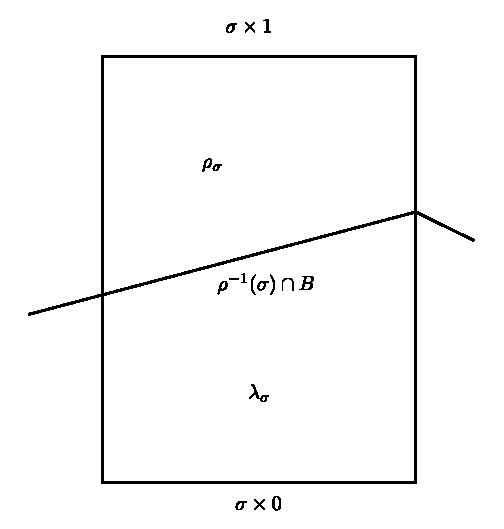
\includegraphics{figure/fig12.eps}
\end{figure}

Now there is an obvious combinatorial isomorphism $\mathscr{C}\approx \mathfrak{a}\times\mathscr{J}$; and if we choose the centerings described we obtain
$h:A\times I\to A\times I$\pageoriginale which is simplicial relative to $d(\mathscr{C},\theta)$ and $d(\mathfrak{a}\times\mathscr{J},\eta)$, and has the desired properties.
\end{proof}

\setcounter{subsection}{12}
\subsection{}\label{chap6-sec6.4.13}
In this situation, define 
$$
\lambda_{B}=\left\{(a,t)\mid a\in A, t\in I, \exists b\in B,b=(a,s),t\leq s\right\}
$$
i.e.\@ this is all the stuff of the left of $B$. Then $h$ takes $\lambda_{B}$ onto $A\times[0,\frac{1}{2}]$, $B$ onto $A\times\frac{1}{2}$. In particular $B$ is collared in $\lambda_{B}$.

\subsection{``Spindle Maps''.}\label{chap6-sec6.4.14}
Let $L\subset A$, with the cone on $L$ and vertex `$a$' contained in $A$. Call the cone $S$. Suppose $S-L$ is open in $A$ (This is the case when a is a vertex of a simplicial presentation $\mathfrak{a}$ of $A$, and $L=|Lk(a,\mathfrak{a})|$ and $S=|St(a,\mathfrak{a})|$.

Let $\beta=I\to I$ be an imbedding with $\beta(1)=1$. In this situation we define the ``{\em spindle map}''.
$$
m(\beta,L,a):A\times I\to A\times I
$$
thus: on $L\ast[a\times I]$, it is the join of the identity map on $L$ with the map $(a,t)\to (a,\beta(t))$ of $a\times I$. On the rest of $A\times I$ it is the identity map.

A spindle map $m$ is an embedding, and commutes with the projection on $A$. If $B$ is a cross section of $A\times I$ which does not intersect $A\times 1$, then $m(B)$ has these properties also.

\setcounter{proposition}{16}
\begin{proposition}\label{chap6-prop6.4.15}
Let $A\subset P$ be polyhedra. If $A$ is locally collared in $P$, then $A$ is collared in $P$.
\end{proposition}

\begin{proof}
In $P\times[0,1]$, consider the subpolyhedron $Q=P\times 0\cup A\times[0,1]$. We identify $P$ with $P\times 0\subset Q$. Let $\mathscr{P}$ be a simplicial presentation of $P$, in which a subpresentation $\mathfrak{a}$ covers\pageoriginale $A$.

Consider a vertex `$a$' of $\mathfrak{a}$; let $L_{A}$ and $L_{P}$ denote $|Lk(a,\mathfrak{a})|$ and $|Lk(a,\break\mathscr{P})|$. Then $(L_{P},L_{A})$ is a link of $a$ in $(P,A)$ and there is a polyhedral equivalence $\gamma:L_{P}\to L_{A}\ast\nu$ for some $v$, taking $L_{A}$ onto $L_{A}$. We can make $\gamma$ identity on $L_{A}$ by composing with $(\lambda|L_{A})^{-1}\ast \text{id}_{\nu}$. And so we suppose $\gamma/L_{A}$ is identity.

We can suppose that $v$ is so situated (for example in a larger vector space) that $L_{A}\ast v$ and $L_{A}\ast(a,1)$ intersect only in $L_{A}$. Thus we have via $\gamma$ and the identity on $L_{A}\ast(a,1)$, a polyhedral equivalence of $L_{Q}=L_{P}\cup L_{A}\ast(a,1)$ with $L_{A}\ast E$ where $E=\{v,(a,1)\}$, which is identity on $L_{A}\ast(a,1)$. Now $L_{Q}\ast a$ is a star of `$a$' in $Q$, and via this p.e.\@ is polyhedrally equivalent to $L_{A}\ast E\ast a$.
We can find a polyhedral equivalence $\beta$ of $E\ast a$ (which is equivalent to a closed $1$-cell) leaving $v$ and $(a,1)$ fixed and taking $(a,0)$ to $(a,\frac{1}{2})$. Such a obviously takes $a\times [0,1]$ onto $a\times [\frac{1}{2},1]$.

\begin{figure}
\centering
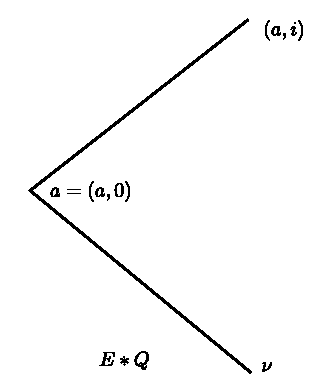
\includegraphics{figure/fig13.eps}
\end{figure}

Take the join of $\beta$ and the identity map $L_{A}$, this gives a polyhedral equivalence of $L_{Q}\ast a$ which is the identity on $L_{Q}$. Hence this can be extended to a polyhedral equivalence of $Q$ by identity outside $L_{Q}\ast a$. Let us call this equivalence of $Q$,\pageoriginale $\beta_{a}\cdot \beta_{a}(A\times I)\subset A\times I$, and $\beta_{a}|A\times I$ is a spindle map.

Now take the composition $h$ in any order of all such $\beta_{a}$, with `$a$' running over all the vertices of $\mathfrak{a}$. This maps $A=A\times 0$ into a cross section $h(A)=B$ of $A\times[0,1]$ which does not intersect $A\times 1$ or $A\times 0$. Finally $h(P)\cap A\times I=\lambda B$.

$B$ is collared in $\lambda B$, and so in $h(P)$. Then, taking $h^{-1}$ we see that $A$ is collared in $P$.
\end{proof}

\setcounter{proposition}{15}
\begin{corollary}\label{chap6-coro6.4.16}
If $M$ is a P.L.\@ Manifold with boundary $M$, then $\p M$ is collared in $M$.
\end{corollary}

Now, an application of the corollary:

\begin{proposition}\label{chap6-prop6.4.17}
If $h$ is an isotopy of $\p M$, then $h$ extends to an isotopy $H$ of $M$.
\end{proposition}

\begin{proof}
Let $\beta :I\times I\to I$ be the map given by $\beta(s,t)=\Max(t-s,0)$. This is polyhedral, e.g.\@ the diagram shows that triangulations and the images of the vertices.
\begin{figure}[H]
\centering
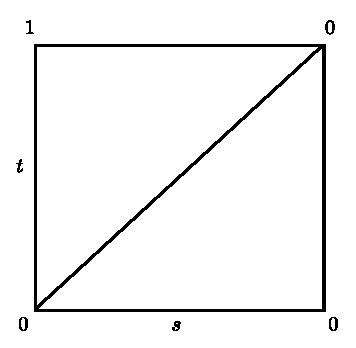
\includegraphics{figure/fig14.eps}
\end{figure}

$\beta(s,0)=0$, $\beta(1,t)=0$, $\beta(0,t)=t$. Define $H=(\p M\times I)\times I\to (\p M\times I)\times I$ by $H((x,s),t)=((h_{\beta(s,t)}(x),s),t)$. This is polyhedral.
$$
H((x,s),0)=((h_{\beta(s,0)}(x),s),0)=((x,s),0),
$$
since $h_{0}=\Id$. Hence $H_{0}=\Id$ of $\p M\times I$.
$$
H((x,0),t)=((h_{\beta(0,t)}(x),0),t)=((h_{t}(x),0),t).
$$

Thus $H$ extends the isotopy $\p M\times 0$ given by $h$ (identifying $\p M$ and $\p M\times 0$). And\pageoriginale
\begin{align*}
H((x,1),t) &= ((h_{\beta(1,t)}(x),1),t)\\
&= ((x,1),t)\quad\text{since}\quad \beta(1,t)=0.
\end{align*}

Hence $H|\p M\times 1$ is identity. Hence the isotopy $h$ of $\p M$ extends to an isotopy $H$ of any collar so that at the upper end of the collar it is identity again, and therefore it can be extended inside. Thus $h$ extends to an isotopy of $M$.
\end{proof}

\section[Absolute Regular Neighbourhoods and some...]{Absolute Regular
  Neighbourhoods and some\hfil\break Newmanish Theorems}\label{chap6-sec6.5} 

\begin{definition}\label{chap6-defi6.5.1}
A pair of a polyhedra $(P,A)$ is said to be an {\em absolute regular neighbourhood} of a polyhedron $X$, if
\begin{itemize}
\item[(i)] $X\subset P-A$

\item[(ii)] $P\times 0$ is a regular neighbourhood of $X\times 0$ in $P\times 0\cup A\times[0,1]\subset P\times[0,1]$.
\end{itemize}

Hence $A$ is collared in $P$.
\end{definition}

Probably, it will be more natural to consider $X$, $P$ and $A$ in an ambient polyhedron $M$ in which $P$ is a neighbourhood of $X$ as in links and stars. But, after the definition of regular neighbourhood, absolute regular neighbourhood is just a convenient name to use in some tricky situations.

\begin{ex}\label{chap6-ex6.5.2}
If $(P,A)$ is an absolute regular neighbourhood of $X$ and if $h:P\to P'$ is a polyhedral equivalence, then $(P',h\ A)$ is an absolute regular neighbourhood of $h\ X$.
\end{ex}

\begin{ex}\label{chap6-ex6.5.3}
If $N$ is a regular neighbourhood of $X$ in $P$, and $B=Bd_{P}N$, then $(N,B)$ is an absolute regular neighbourhood of $X$.
\end{ex}

\begin{ex}\label{chap6-ex6.5.4}
Let\pageoriginale $P\subset Q$, and suppose that $(P,A)$ is an absolute regular neighbourhood of $X$, and $P-A$ is open in $Q$, and $A$ is locally collared in $Q-(P-A)$. Then $P$ is regular neighbourhood of $X$ in $Q$.
\end{ex}

\begin{ex}\label{chap6-ex6.5.5}
Let $C(A)$ be the cone on $A$ with vertex $v$. Then $(C(A),A)$ is an absolute regular neighbourhood of $v$.
\end{ex}

In particular if $D$ is an $n$-cell, $(D,\p D)$ is an absolute regular neighbourhood of any point $x\in D-\p D$.

\begin{theorem}\label{chap6-thm6.5.6}
If $D$ is an $n$-cell, $M$ a $PL$-manifold, $D\subset\Int M$, then $D$ is a regular neighbourhood of any $x\in D-\p D$ in $M$.
\end{theorem}

\begin{corollary}\label{chap6-coro6.5.7}
If $D$ is an $n$-cell in an $n$-sphere $S$, then $\overline{S-D}$ is an $n$-cell.
\end{corollary}

\smallskip
\noindent
{\bf Proof of the theorem:}~ The proof of the theorem is by induction on the dimension of $M$; we assume the theorem as well as the corollary for $n-1$.
\begin{itemize}
\item[(i)] First we must show that $D-\p D$ is open in $M$. If we look at the links, this would follow if we know that a polyhedral imbedding of an $(n-1)$-sphe
re in an $(n-1)$-sphere is necessarily onto. And this can be easily seen by looking at the links again and induction. (see \ref{chap4-sec4.4} in particular \ref{chap4-prop4.4.14} and \ref{chap4-ex4.4.17}(a)).

\item[(ii)] If we know that $\p D$ is collared in $M-\text{int\,}D$ (it is collared in $D$), we are through by \ref{chap6-ex6.5.4}. For this, it is enough to show that $\p D$ is locally collared in $M-\text{int\,}D$. Consider a link of $a$ in $M$, say $S^{n-1}$, such that a link of `$a$' in $D$ is an\pageoriginale $(n-1)$-cell $D^{n-1}_{a}\subset S^{n-1}_{a}$, with $D^{n-1}_{a}\cap \p D=\p D^{n-1}_{a}$. It is clearly possible to choose such links (see \ref{chap4-ex4.4.17}(b)). Now, a link of `$a$' in $M-\text{int\,}D$ is $S^{n-1}_{a}-(D^{n-1}_{a}-\p D^{n-1}_{a})$. As in (i) $D^{n-1}_{a}-\p D^{n-1}_{a}$ is open in $S^{n-1}_{a}$ and therefore the link of $a$ in $M-\text{int\,}D$ is $\overline{S^{n-1}_{a}-D^{n-1}_{a}}$. But by the 
corollary to the theorem in the $(n-1)$-case, this is an $(n-1)$-cell, say $\Delta^{n-1}$ and it meets $D$ in $\p D^{n-1}_{a}=\p \Delta^{n-1}$. And $(\Delta^{n-1},\p \Delta^{n-1})$ is equivalent to $(C(\p \Delta^{n-1}),\p \Delta^{n-1})$. Therefore $\p D$ is locally collared in $M-\text{int\,D}$ and we are through.
\end{itemize}

\smallskip
\noindent
{\bf Proof of the corollary assuming the theorem:}~ Represent $S^{n}$, a standard $n$-sphere as a suspension of $S^{n-1}$, a standard $(n-1)$-sphere, and observe that the lower hemisphere (say $D_{s}$) is a regular neighbourhood of the south pole, say $s$. Let $f$ be a polyhedral equivalence of $S$ to $S^{n}$ taking a point $x\in D-\p D$ to the south pole $s$. By the theorem $D$ is a regular neighbourhood of $x$, therefore $f(D)$ is a regular neighbourhood of the $s$ in $S^{n}$. By \ref{chap6-prop6.3.2} there is a polyhedral equivalence $p$ of $S^{n}$ such that $p(D_{s})=f(D)$. Therefore $f(\overline{S-D})=\overline{f(S)-f(D)}=\overline{S^{n}-p(D_{s})}=\overline{p(S^{n})-p(D_{s})}=\overline{p(S^{n}-D_{s})}=p(D_{n})$, where $D_{n}$ denotes the upper hemisphere. Therefore $p^{-1}\cdot f(\overline{S-D})=D_{n}$ or $\overline{S-D}$ is a $n$-cell.

\begin{excoro}\label{chap6-ex6.5.8}
If $M$ is a $PL$ $n$-manifold and $D_{1}$, $D_{2}$ are two $n$-cells contained in the interior of the same component of $M$, then there is an isotopy $h$ of the identity map of $M$, such that $h(D_{1})=D_{2}$.
\end{excoro}

We\pageoriginale usually express this by saying that ``any two $n$-cells in the interior of the same component of $M$ are equivalent'' or that they are ``equivalent by an isotopy of $M$''.

If $M$ is a $PL$ $n$-manifold, $\p M$ its boundary, then by \ref{chap6-ex6.5.8}, any two $(n-1)$-cells in the same component of $\p M$ are equivalent by an isotopy of $\p M$. Since this is actually an isotopy of the identity, by \ref{chap6-prop6.4.17} we can extend it to $M$. Thus

\begin{proposition}\label{chap6-prop6.5.9}
Any two $(n-1)$-cells in the same component of $\p M$ are equivalent by an isotopy of $M$.
\end{proposition}

This immediately gives

\begin{ex}\label{chap6-ex6.5.10}
If $D$ is an $n$-cell and $\Delta$ an $(n-1)$-cell in $\p D$, then $(D,\Delta)$ is a cone pair (That is, there is a polyhedral equivalence of $(D,\Delta)$ and $(C(\Delta),\Delta)$. And we have seen such a polyhedral equivalence can be assumed to be identity on $\Delta$).
\end{ex}

This can also be formulated as:

\medskip
\noindent{\textbf{Ex. 6.5.10$^1$}}
If $\Delta_{i}$ is an $(n-1)$-cell in the boundary of $D_{i}$, an $n$-cell, $i=1,2$, any polyhedral equivalence $\Delta_{1}\to \Delta_{2}$ can be extended to a polyhedral equivalence $D_{1}\to D_{2}$.

Also from \ref{chap6-prop6.5.9}, it is easy to deduce if $\Delta$ is any $(n-1)$-cell in $\p M$, then there is at least one $n$-cell $D$ in $M$ such that $D\cap \p M=\Delta \subset \p D$. From this follows the useful proposition:

\begin{ex}\label{chap6-ex6.5.11}
If $M$ is a $PL$ $n$-manifold and $D$ an $n$-cell with $M\cap D=\p M\cap \p D=$ an $(n-1)$-cell, then $M\cup D$ is polyhedrally equivalent to $M$. Moreover, the polyhedral equivalence can be chosen to be identity outside any given neighbourhood of $M\cup D$ in $M$.
\end{ex}

The\pageoriginale methods of the proof of the theorem \ref{chap6-thm6.5.6}, can be used to prove the following two propositions, which somewhat clarify the nature of regular neighbourhoods in manifolds:

\begin{ex}\label{chap6-ex6.5.12}
Let $M$ be a $PL$-manifold, $\p M$ its boundary (possibly $\emptyset$), and $N$ a regular neighbourhood of $X$ in $M$. Then
\begin{itemize}
\item[(a)] $N$ is a $PL$-manifold with (non-empty) boundary unless $X$ is a union of components of $M$.

\item[(b)] If $X\subset M-\p M$, then $N\subset M-\p M$, the interior of $M$.

\item[(c)] If $X\cap \p M\neq \emptyset$, $N\cap \p M$ is a regular neighbourhood of $X\cap \p M$ in $\p M$.

\item[(d)] In case (c), $Bd_{M}N$ is an $(n-1)$-manifold, meeting $\p M$ in an $(n-2)$-manifold $\p N'$, where $N'=N\cap \p M$.
\end{itemize}

[Note that $\text{int}_MN$ and $bd_{M}N$ denote the interior and boundary of $N$ in the topology of $M$. On the otherhand if $N$ is a $PL$-manifold int $N$ and $\p N$ denotes the sets of points of $N$ whose links are spheres and cells respectively].

Hint: Use \ref{chap4-ex4.4.8}.
\end{ex}

\begin{ex}\label{chap6-ex6.5.13}
If $N$ is a regular neighbourhood of $X$ in $M$, a $PL$-manifold with $X\subset \text{int\,}M$, and $N'$ is polyhedrally equivalent to $N$ and located in the interior of a $PL$-manifold $M_{2}$ of the same dimension as $M$, then $N'$ is a regular neighbourhood of $X'$ in $M_{2}$, where $X'$ is the image of $X$ under the polyhedral equivalence $N\to N'$.
\end{ex}

\begin{ex}\label{chap6-ex6.5.14}
A\pageoriginale is any polyhedron, and $I$ the standard $1$-cell $(A\times I,A\times 1)$ is an absolute regular neighbourhood of $A\times 0$. If $0< \mathcal{L}<1$, then $(A\times I,A\times\{0,1\})$ is an absolute regular neighbourhood of $A\times \mathcal{L}$.
\end{ex}

\begin{ex}\label{chap6-ex6.5.15}
The union of two $n$-manifolds intersecting in an $(n-1)$ submanifold of their boundaries is an $n$-manifold.
\end{ex}

\section{Collapsing}\label{chap6-sec6.6}

\begin{definition}\label{chap6-defi6.6.1}
Let $\mathscr{P}$ be a regular presentation. {\em A free edge} of $\mathscr{P}$ is some $E\in\mathscr{P}$ such that there exists one and only one $A\in\mathscr{P}$ with $E<A$. We may term $A$ the {\em attaching membrane} of the free edge $E$. It is clear that $A$ is not in the boundary of any other element of $\mathscr{P}$; for if $A<B$, then $E<B$. It is easily proved that $\dim A=1+\dim E$.
\end{definition}

The set $\mathscr{P}-\{E,A\}$ is again a regular presentation, and is said to be obtained from $\mathscr{P}$ by an {\em elementary collapse} at the free edge $E$.

\begin{definition}\label{chap6-defi6.6.2}
We say that a polyhedral presentation $\mathscr{P}$ {\em collapses} ({\em combinatorially}) {\em to} a polyhedral presentation $\mathcal{Q}$, and write $\mathscr{P}\searrow \mathcal{Q}$, if there exists a finite sequence of presentations
$$
\mathscr{P}_{1},\ldots,\mathscr{P}_{k}\quad\text{with}\quad \mathscr{P}=\mathscr{P}_{1}\quad\text{and}\quad \mathscr{P}_{k}=\mathcal{Q}
$$
and cells $E_{1},\ldots,E_{k-1}$, $E_{i}\in\mathscr{P}_{i}$ s.t.\@ $\mathscr{P}_{i}$ is obtained from $\mathscr{P}_{i-1}$ be an elementary collapse at $E_{i-1}$.
\end{definition}

\begin{proposition}\label{chap6-prop6.6.3}
If $\mathcal{Q}$ is obtained from $\mathscr{P}$ by an elementary collapse at $E$; and if $\mathscr{P}'$ is obtained from $\mathscr{P}$ by bisecting a cell\pageoriginale $C$ by a bisection of space $(L;H+,H-)$ and if $\mathcal{Q}'\subset \mathscr{P}'$ is the subpresentation with $|\mathcal{Q}'|=|\mathcal{Q}|$, then $\mathscr{P}'\searrow \mathcal{Q}'$. [Remark: Recall that, we have been always dealing with Euclidean polyhedra].
\end{proposition}

\begin{proof}
If the bisection is trivial there is nothing to prove, so suppose that the bisection is non trivial. Then there are three cases.

\medskip
\noindent
{\bf Case (i)} $C$ is neither $E$ nor $A$. In this case, $E$ is a free edge of $\mathscr{P}'$ with attaching membrane $A$, and $\mathcal{Q}'=\mathscr{P}'-\{E,A\}$; thus $\mathcal{Q}'$ is obtained from $\mathscr{P}'$ by an elementary collapse. 

\medskip
\noindent
{\bf Case (ii)} $C=E$. Define $E_{1}=H+\cap E$, $E_{2}=H-\cap E$, $F=L\cap E$. Then we have
\[
\xymatrix@=.15cm{
 & E_{1}\ar@{{}>}[dl] &\\
F & & A\ar@{{}>}[ul]\ar@{{}>}[dl]\\
& E_{2}\ar@{{}>}[ul] & 
}
\]
and no other cells of $\mathscr{P}'$ are greater than $F$, $E_{1}$, $E_{2}$ or $A$.
\begin{figure}[H]
\centering
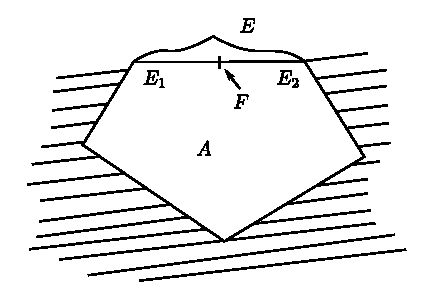
\includegraphics{figure/fig15.eps}
\end{figure}

Thus $E_{1}$ is a free edge of $\mathscr{P}'$ with attaching membrane $A$; $F$ is a free edge of $\mathscr{P}'-\{E_{1},A\}$ with attaching membrane $E_{2}$. The result of these two elementary collapses is $\mathcal{Q}=\mathcal{Q}'$.

\medskip
\noindent
{\bf Case (iii)} $C=A$\pageoriginale

Define $A_{1}=H+\cap A$, $A_{2}=H-\cap A$, $B=L\cap A$. Now $\p A_{1}\cup \p A_{2}$ contains $\p A$, and therefore either $\p A_{1}$ or $\p A_{2}$ intersects $E$; say, $\p A_{1}\cap E\neq \emptyset$. Then $\mathscr{P}'$ being regular, we must have $E<A_{1}$; then for dimensional reasons, $\dim E=\dim B$, we cannot have $E<B$ hence $E\subset H+$; and so it is impossible to have $E<A_{2}$. In summary, $E<A_{1}>B<A_{2}$.
\begin{figure}[H]
\centering
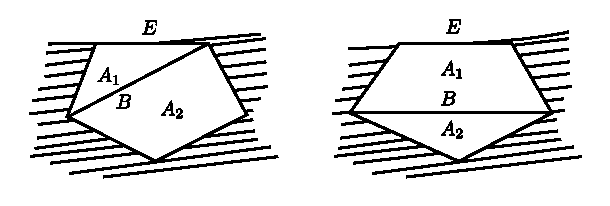
\includegraphics{figure/fig16.eps}
\end{figure}

Thus $E$ is a free face of $\mathscr{P}'$ with attaching membrane $A_{1}$; $B$ is a free face of $\mathscr{P}'-\{E,A_{1}\}$ with attaching membrane $A_{2}$. The result of these two elementary collapses is $\mathcal{Q}'$.
\end{proof}

\begin{proposition}\label{chap6-prop6.6.4}
If $\mathscr{P}\searrow \mathcal{Q}$, and $\mathscr{P}'$ is obtained from by a finite sequence of bisections of cells, and $\mathcal{Q}'$ is the subpresentation of $\mathscr{P}'$ defined by $|\mathcal{Q}'|=|\mathcal{Q}|$; then $\mathscr{P}'\searrow \mathcal{Q}'$. 
\end{proposition}

\begin{proof}
The proof is by induction, first, on the number of collapses in $\mathscr{P}\searrow \mathcal{Q}$, and second, on the number of bisections involved. The inductive step is \ref{chap6-prop6.6.3}.
\end{proof}

\begin{definition}\label{chap6-defi6.6.5}
We say that a polyhedron $P$ {\em collapses (geometrically) to a subpolyhedron} $Q$, if there is a regular presentation $\mathscr{P}$ of $P$ with a subpresentation $\mathcal{Q}$ covering $Q$, such that $\mathscr{P}$ collapses combinatorially to $\mathcal{Q}$. We write $P\searrow Q$.
\end{definition}

This\pageoriginale notion is polyhedrally invariant:

\begin{proposition}\label{chap6-prop6.6.6}
If $P\searrow Q$, and $\alpha:P\to X$ is a polyhedral equivalence, then $X\searrow \alpha(Q)$.
\end{proposition}
$\mathcal{L} \quad  \alpha$
\begin{proof}
There are regular presentations $\mathscr{P}$, $\mathcal{Q}$ of $P$ and $Q$, with $\mathscr{P}\searrow \mathcal{Q}$ combinatorially, and simplicial presentations $\mathscr{S}$, $\mathscr{X}$ of $P$ and $X$ with $\mathcal{L}$ simplicial relative to $\mathscr{S}$ and $\mathscr{X}$. There is a regular presentation $\mathscr{P}'$ of $P$ refining $\mathscr{P}$ and $\mathscr{S}$, and obtained from $\mathscr{P}$ (also from $\mathscr{S}$ but we do not need it in this proposition) by a finite sequence of bisections. Hence if $\mathcal{Q}'$ is the subpresentation of $\mathscr{P}'$ covering $Q$, then $\mathscr{P}'\searrow \mathcal{Q}'$, by \ref{chap6-prop6.6.4}. Since $\mathcal{L}$ is one-to-one and linear on each element of $\mathscr{P}'$, the set $\mathcal{L}(\mathscr{P}')=\{\mathcal{L}(C)\mid C\in \mathscr{P}'\}$ is a regular presentation of $X$, which is combinatorially isomorphic to $\mathscr{P}'$; and $\mathcal{L}(\mathcal{Q}')$ is subpresentation covering $\mathcal{L}(Q)$, which is combinatorially isomorphic to $\mathcal{Q}'$. Threrefore $\mathcal{L}(\mathscr{P})\searrow \mathcal{L}(\mathcal{Q}')$ or $X\searrow (Q)$.
\end{proof}

\begin{proposition}\label{chap6-prop6.6.7}
If $P_{1}\searrow P_{2}$, and $P_{2}\searrow P_{3}$, then $P_{1}\searrow P_{2}$.
\end{proposition}

\begin{proof}
Let $\mathscr{P}_{1}$, $\mathscr{P}_{2}$ be presentation of $P_{1}$, $P_{2}$ with $\mathscr{P}_{1}\searrow \mathscr{P}_{2}$, and $\mathscr{P}_{3}$, $\mathscr{P}_{4}$ be presentations of $P_{2}$, $P_{3}$ with $\mathscr{P}_{3}\searrow \mathscr{P}_{4}$. By 1.10.6 there is a regular refinement $\mathcal{Q}$ of $\mathscr{P}_{1}\cup \mathscr{P}_{2}\cup \mathscr{P}_{3}\cup \mathscr{P}_{4}$, and subpresentations $\mathcal{Q}_{1}$, $\mathcal{Q}_{2}$, $\mathcal{Q}_{3}$, $\mathcal{Q}_{4}$ of with $|\mathscr{P}_{i}|=|\mathcal{Q}_{i}|$, $\mathcal{Q}_{i}$ obtained from $\mathscr{P}_{i}$ by a sequence of bisections. Clearly $\mathcal{Q}_{2}=\mathcal{Q}_{3}$ and by \ref{chap6-prop6.6.4}, $\mathcal{Q}_{1}\searrow \mathcal{Q}_{2}$, and $\mathcal{Q}_{3}\searrow \mathcal{Q}_{4}$ and therefore $P_{1}\searrow P_{2}$.
\end{proof}

\begin{proposition}\label{chap6-prop6.6.8}
If $N$ is a regular neighbourhood of $X$ in $P$, then $N\searrow X$.
\end{proposition}

\begin{proof}
By\pageoriginale virtue of \ref{chap6-prop6.6.6} and the definition of regular neighbourhood, it is enough to look at any particular $N$. Let $\mathscr{P}$ be a simplicial presentation of $P$ with a full subpresentation $\mathscr{X}$ covering $X$; and let $\varphi:P\to [0,1]$ be the usual map. Take $N=\varphi^{-1}([0,\frac{1}{2}])$.

Let $\sum$ denote all the simplexes of $\mathscr{P}$ having vertices both in $\mathscr{X}$ and $(\mathscr{P}-\mathscr{X})$. We prove $N\searrow X$ by induction on the number of elements of $\sum$. If $\sum=\emptyset$, then $N=X$, and there is nothing to do. Hence we can start the induction.

Let
\begin{align*}
\mathscr{N} &= \mathscr{X}\cup \{\sigma\cap \varphi^{-1}((0,\frac{1}{2}))\mid \sigma\in \sum\}\\
&\quad \cup \{\sigma\cap \varphi^{-1}(\frac{1}{2})\mid \sigma\in\sum\}
\end{align*}

Then $\mathscr{N}$ is a regular presentation of $N$. If $\sigma$ is an element of of maximal dimension, $\sigma\cap \varphi^{-1}(\frac{1}{2})$ is a free edge of $\mathscr{N}$ with attaching membrane $\sigma\cap \varphi^{-1}((0,\frac{1}{2}))$. (Note that $\sigma$ is a {\em principal} simplex of $\mathscr{P}$ i.e. not the face of any other simplex). After doing the elementary collapse we are left with $\mathscr{N}'$. Now $\mathscr{P}-\{\sigma\}=\mathscr{P}'$ is a regular presentation containing $\mathscr{X}$, and the corresponding $\sum'=\sum-\{\sigma\}$. Hence inductively $\mathscr{N}'\searrow \mathscr{X}$. And so, $\mathscr{N}\searrow \mathscr{X}$.
\end{proof}

\begin{ex}\label{chap6-ex6.6.9}
Let $N'$ be a neighbourhood of $X$ in $P$, (all polyhedra). If $N'\searrow X$, then there is a regular neighbourhood $N$ of $X$ in $P$, $N\subset \Int_{P}N'$ such that $N'\searrow N$.
\end{ex}

\section{Homogeneous Collapsing}\label{chap6-sec6.7}

Let $\mathscr{P}$ be a regular presentation, with $E$, $A\in \mathscr{P}$, $E<A$ and $\dim A=\dim E+1$.

\setcounter{pageoriginal}{144}
Recall the definition of $\lambda_{\mathscr{P}}E$. This is defined, relative\pageoriginale to some centering $\eta$ of $\mathscr{P}$, to be the full subpresentation of $d\mathscr{P}$ whose vertices are, $\{\eta \mathscr{C}\mid E<C\in\mathscr{P}\}$. 

\begin{definition}\label{chap6-defi6.7.1}
Let $E$, $A$, $\mathscr{P}$; be as above and $\eta$ be a centering of $\mathscr{P}$. $(E,A)$ is said to be {\em homogenous} in $\mathscr{P}$, if there is a polyhedron $X$ and a polyhedral equivalence $f:|\lambda_{\mathscr{P}}E|\to X\ast\{u,w\}$ a suspension of $X$, such that $f(\eta A)=w$.
\end{definition}

It is easily seen that if this is true for one centering of $\mathscr{P}$, then it is true for any other centering of $\mathscr{P}$; hence ``$(E,A)$ is homogeneous in $\mathscr{P}$'' is well defined.

\begin{definition}\label{chap6-defi6.7.2}
Let $\mathscr{X}\subset \mathscr{N}$ be subpresentations of $\mathscr{P}$. We say that {\em $\mathscr{N}$ collapses to $\mathscr{X}$ homogeneously (combinatorially) in $\mathscr{P}$}, if there is a finite sequence of subpresentations of $\mathscr{P}$,
$$
\mathscr{N}_{1},\ldots,\mathscr{N}_{k}
$$
and pairs of cells $(E_{1},A_{1}),\ldots,(E_{k-1},A_{k-1})$, $E_{i}$, $A_{i}\leftarrow \mathscr{N}_{i}$ such that 
\begin{itemize}
\item[(1)] $\mathscr{N}_{1}=\mathscr{N}$, $\mathscr{N}_{k}=\mathscr{X}$

\item[(2)] $\mathscr{N}_{i+1}$ is obtained from $\mathscr{N}_{i}$ by an elementary collapse at $E_{i}$, a free edge of $\mathscr{N}_{i}$ with attaching membrane $A_{i}$, for $i=1,\ldots,k-1$ and

\item[(3)] $(E_{i},A_{i})$ is homogeneous in $\mathscr{P}$, for $i=1,\ldots,k-1$. 
\end{itemize}
\end{definition}

\begin{proposition}\label{chap6-prop6.7.3}
If $\mathscr{P}'$ is obtained from $\mathscr{P}$ by bisecting a cell $C$ by a bisection of space $(L;H+,H-)$: and if $\mathscr{X}\subset \mathscr{N}\subset \mathscr{P}$, with $\mathscr{X}$ obtained from $\mathscr{N}$ by an elementary collapse at a free edge $E$ with attaching membrane $A$, where $(E,A)$ is homogeneous in $\mathscr{P}$; and if $\mathscr{N}'$, $\mathscr{X}'$ are the subpresentations of $\mathscr{P}'$ covering $|\mathscr{N}|$ and\pageoriginale $|\mathscr{X}|$; then $\mathscr{N}'\searrow \mathscr{X}'$ homogeneously in $\mathscr{P}'$.
\end{proposition}

\begin{proof}
If the bisetion in trivial there is nothing to prove. If it is not trivial, there are three cases as in the proof of proposition \ref{chap6-prop6.6.3}.

\medskip
\noindent
{\bf Case 1:}~ $C$ is neither $E$ nor $A$. In this case the only problem is to show that $(E,A)$ is homogeneous in $\mathscr{P}'$. Let us suppose that everything is occuring in a vector space $V$ of $\dim n$; and let $\dim E=k$. Then there is an orthogonal linear manifold $M$ of dimension $(n-k)$, intersecting $E$ in a single point $\eta(E)=e$, say. It is fairly easy to verify that in such a situation if $E<D$, then $D\cap M\neq \emptyset$.

If we now choose centerings of $\mathscr{P}$ and $\mathscr{P}'$ so that whenever $D\cap M\neq \emptyset$, we have the center of $D$ belonging to $M$, then defining
$$
\mathcal{Q}=\{D\cap M\mid D\cap M\neq \emptyset, D\in \mathscr{P}\}
$$
and $\mathcal{Q}'$ similarly with respect to $\mathscr{P}'$, we will have:
\begin{align*}
\lambda_{\mathscr{P}}(E) &= \lambda_{\mathcal{Q}}(e)\\
\lambda_{\mathscr{P}'}(E) &= \lambda_{\mathcal{Q}'}(e).
\end{align*}
and $\mathcal{Q}$, $\mathcal{Q}'$ are regular presentations of $|\mathscr{P}|\cap M$. Hence both $|\lambda_{\mathscr{P}}(E)|$ and $|\lambda_{\mathscr{P}'}(E)|$ are links of $e$ in $|\mathscr{P}|\cap M$, and hence polyhedrally equivalent (by an approximation to the standard mistake); if we choose a center of $A$ the same in both case, we get a polyhedral equivalence taking $\eta A$ to $\eta A$. Finally, by hypothesis $|\lambda_{\mathscr{P}}(E)|$ is equivalent to a suspension with $\eta A$ as a pole; and so $|\lambda \mathscr{P}'(E)|$ has the same property, and $(E,A)$ is homogeneous in $\mathscr{P}'$.

\medskip
\noindent
{\bf Case 2:}~ $C=E$;\pageoriginale we define $E_{1}$, $E_{2}$, $F$ as in the proof of \ref{chap6-prop6.6.3}. We have to show that $(E_{1},A)$ and $(F,E_{2})$ are homogeneous in $\mathscr{P}'$.

That $(E_{1},A)$ is homogeneous in $\mathscr{P}'$ follows from the fact $|\lambda_{\mathscr{P}}(E)|=|\lambda_{\mathscr{P}'}(E_{1})|$ (with appropriate centerings) because any $D>E_{1}$ in $\mathscr{P}'$ is an element of $\mathscr{P}$ which is $>E_{1}$ and hence, $\mathscr{P}$ being regular $>E$.

That $(F,E_{2})$ is homogeneous in $\mathscr{P}'$, we see by the formula:
$$
\lambda_{\mathscr{P}'}(F)=\lambda_{\mathscr{P}}(E)\ast \{\eta E_{1},\eta E_{2}\}
$$
(calling the appropriate centering of $\mathscr{P}'$ also $\eta$).

\medskip
\noindent
{\bf Case 3:}~ $C=A$; we define $A_{1}$, $A_{2}$, $B$ as in the proof of \ref{chap6-prop6.6.3}. We have to show that $(E,A_{1})$ and $(B,A_{2})$ are homogenous.

There is a simplicial isomorphism $\lambda_{P}(E)\approx \lambda_{\mathscr{P}'}(E)$ taking $\eta(A)$ onto $\eta(A_{1})$. And as $(E,A)$ is homogeneous in $\mathscr{P}$, we have $(E,A_{1})$ is homogeneous in $\mathscr{P}'$.

That $(B,A_{2})$ is homogeneous in $\mathscr{P}'$ we see by a formula like that in case $2$:
$$
\lambda_{\mathscr{P}'}(B)=\lambda_{\mathscr{P}}(A)\ast \{\eta A_{1},\eta A_{2}\}.
$$
\end{proof}

\begin{proposition}\label{chap6-prop6.7.4}
If $\mathscr{N}\searrow \mathscr{X}$ homogeneously in $\mathscr{P}$, and $\mathscr{P}'$ is obtained from $\mathscr{P}$ by a finite sequence of bisections of space, and $\mathscr{N}'$, $\mathscr{X}'$ are the subpresentations of $\mathscr{P}'$ covering $|\mathscr{N}|$ and $|\mathscr{X}|$, then $\mathscr{N}'\searrow \mathscr{X}'$ homogeneously in $\mathscr{P}'$.

This follows from \ref{chap6-prop6.6.3}, as \ref{chap6-prop6.6.4} from \ref{chap6-prop6.6.3}. 
\end{proposition}

\begin{definition}\label{chap6-defi6.7.5}
Let $P$ be a polyhedron, and $X$, $N$ subpolyhedra of\pageoriginale $P$. $N$ is said to {\em collapse homogeneously (geometrically) to $X$ in $P$}, if there are regular presentation $\mathscr{X}\subset \mathscr{N}\subset \mathscr{P}$ covering $X$, $N$ and $P$ respectively such that $\mathscr{N}$ collapses homogeneously to $\mathscr{X}$ combinatorially in $\mathscr{P}$.

We write {\em $N\searrow X$ homogeneously} in $P$. This definition is again polyhedrally invariant:
\end{definition}

\begin{proposition}\label{chap6-prop6.7.6}
If $N\searrow X$ homogeneously in $P$, and $\mathcal{L}:P\to Q$ is a polyhedral equivalence, then $\mathcal{L}(N)\to \mathcal{L}(X)$ homogeneously in $Q$.

This follows from \ref{chap6-prop6.7.4} as \ref{chap6-prop6.6.6} from \ref{chap6-prop6.6.4}.
\end{proposition}

\begin{proposition}\label{chap6-prop6.7.7}
If $N$ is a regular neighbourhood of $X$ in $P$, then $N\searrow X$ homogeneously in $P$.
\end{proposition}

\begin{proof}
As in \ref{chap6-prop6.6.8}, we start with a simplicial presentation $\mathscr{P}$ of $P$ in which a full subpresentation $\mathscr{X}$, covers $X$, and take $N=\varphi^{-1}([0,\frac{1}{2}])$ where $\varphi:P\to [0,1]$ is the usual map. By virtue of \ref{chap6-prop6.7.6}, and the definition of regular neighbourhood, it is enough to prove that this $N\searrow X$ homogeneously.

Let $\mathscr{N}$ be the regular presentation of $N$ consisting of cells of the form:
\begin{align*}
& \text{simplexes of~ }\mathscr{X}\\
& \sigma\cap \varphi^{-1}((0,\frac{1}{2})),\quad\text{for}\quad \sigma\in \mathscr{P}\quad\text{with}\quad \varphi(\sigma)=(0,1)\\
& \sigma\cap \varphi^{-1}(\frac{1}{2}),\quad\text{for}\quad \sigma\in \mathscr{P}\quad\text{with}\quad \varphi(\sigma)=(0,1)
\end{align*}

Define $\mathscr{P}'$ to consist of
\begin{align*}
&\text{all simplexes of~ }\mathscr{X},\\
&\text{all simplexes of $\mathscr{P}$ which have no vertices in } \mathscr{X}.\\
& \left.
 \begin{aligned}
&\sigma\cap \varphi^{-1}((0,\frac{1}{2}))\\
 &\sigma\cap \varphi^{-1}((\frac{1}{2}))\\
&\sigma\cap \varphi^{-1}(\frac{1}{2},1)
  \end{aligned} \right\}
\text{~ for~ } \sigma\in \mathscr{P}\quad\text{with}\quad \varphi(\sigma)=(0,1)
\end{align*}\pageoriginale
$\mathscr{P}'$ is a regular presentation of $P$ which refines $\mathscr{P}$, and has as subpresentations $\mathscr{N}$ and $\mathscr{X}$. $\mathscr{N}$ and $\mathscr{X}$ are the same as in proposition \ref{chap6-prop6.6.8}, and therefore we know that $\mathscr{N}\searrow \mathscr{X}$. Now, the claim is $\mathscr{N}\searrow \mathscr{X}$ homogeneously in $\mathscr{P}'$. In otherwords, if $E=\sigma\cap \varphi^{-1}(\frac{1}{2})$, $A=\sigma\cap \varphi^{-1}((0,\frac{1}{2}))$, where $\sigma\in\mathscr{P}$ with $\varphi(\sigma)=(0,1)$, we have to show that $(E,A)$ is homogeneous in $\mathscr{P}'$. In fact denoting by $\mathscr{B}$ the subpresentation of $\mathscr{P}'$ covering $\varphi^{-1}(\frac{1}{2})$, we have
\begin{align*}
\lambda_{\mathscr{P}'}(E) &= \lambda_{\mathscr{B}}(E)\ast \{\eta A,\eta A'\},\quad\text{where}\\
A' &= \sigma\cap \varphi^{-1}((\frac{1}{2},1)).
\end{align*}
\end{proof}

\section{The Regular Neighbourhood Theorem}\label{chap6-sec6.8}

We have seen that if $N$ is a regular neighbourhood of $X$ in $P$, then
\begin{itemize}
\item[(1)] $X\subset \text{int\,}_{P}N$

\item[(2)] $N$ is bicollared in $P$

\item[(3)] $N\searrow X$ homogeneously in $P$.
\end{itemize}

Conversely.

\subsection{The Regular Neighbourhood Theorem}\label{chap6-sec6.8.1}

\phantom{a}~

If $X$ $N$ $P$ are polyhedra such that 
\begin{itemize}
\item[(1)] $X\subset \text{int\,}_{P}N$

\item[(2)] $N$ is bicollared in $P$

\item[(3)] $N\searrow X$\pageoriginale homogeneously in $P$
\end{itemize}
\noindent
then $N$ is a regular neighbourhood of $X$ in $P$.

The proof will start with some technicalities which exploit the homogeneity of the collapsing (The $X$'s, $P$'s etc.\@ occuring mean-while should not be confused with the $X$, $P$ of the theorem).

\setcounter{proposition}{1}
\begin{proposition}\label{chap6-prop6.8.2}
Let $Y\subset X$ be polyhedra, and let $P=X\ast\{v,w\}$ a suspension of $X$. Then a regular neighbourhood of $Y\ast v$ in $P$ is a regular neighbourhood of $v$ in $P$. [In other words, a regular neighbourhood of a subcone of a suspension is a regular neighbourhood of one of the poles].
\end{proposition}

\begin{proof}
Let $C_{1}(X)$ denote $X\ast v$ and let $\varphi:C_{1}(X)\to [0,1]$ be the join of the maps $X\to 1$ and $v\to 0$. For any $Z\subset X$, $C_{\mathcal{L}}(Z)$ for $0<\mathcal{L}<1$ will denote the set of points $\{(1-t)v+tz\mid z\in Z,0\leq t\leq \mathcal{L}\}$. If $Z$ is a subpolyhedron $C_{\mathcal{L}}(Z)=(Z\ast v)\cap \varphi^{-1}([0,\mathcal{L}])$. 


By \ref{chap6-ex6.3.7}, it is enough to prove the proposition for some regular neighbourhood of $X\ast v$. Hence, by a couple of maps, it is enough to show that $C_{5/8}(X)$ is a regular neighbourhood of $C_{\frac{1}{2}}(Y)$ in $C_{1}(X)$. (It is clearly a regular neighbourhood of $v$ in $C_{1}(X)$).

Let $\mathscr{X}$ be a simplicial presentation of $X$, containing a subpresentation $\mathscr{Y}$ covering $Y$. We define a regular presentation of $C_{1}(X)$ to consist of:
\begin{align*}
& \{v\}_{\sigma}\quad\text{for}\quad \sigma\in\mathscr{X}\\
& \sigma\{v\}\quad\text{for}\quad \sigma\in \mathscr{X}-\mathscr{Y}\\
& \left.
\begin{array}{l}
\sigma\{v\}\cap \varphi^{-1}((0,\frac{1}{2}))\\
\sigma\{v\}\cap \varphi^{-1}(\frac{1}{2})\\
\sigma\{v\}\cap \varphi^{-1}(\frac{1}{2},1)
\end{array}\right\}\quad\text{for}\quad \sigma\in \mathscr{Y}
\end{align*}\pageoriginale

Then $\mathscr{P}$ has a subpresentation $\mathcal{Q}$ covering $\subset \frac{1}{2}(Y)$, and for each $A\in\mathscr{P}-\mathcal{Q}$ with $\overline{A}\cap C_{\frac{1}{2}}(Y)\ne \emptyset$, $\varphi(A)$ includes the interval $(\frac{1}{2},1)$. Choose a centering $\eta$ of $\mathscr{P}$, so that for all $A\in \mathscr{P}-\mathcal{Q}$ with $\overline{A}\cap C_{\frac{1}{2}}(Y)\neq \emptyset$, $\varphi(\eta A)=\frac{3}{4}$.

Then $d(\mathscr{P},\eta)$ has the property that if $\tau$ is a simplex with vertices both in $d\mathcal{Q}$ and in $d\mathscr{P}-d\mathcal{Q}$, then $\varphi(\tau)$ contains $(\frac{1}{2},\frac{3}{4})$,  and $d\mathcal{Q}$ is full in $d\mathscr{P}$. Choose a centering $\theta$ of $d\mathscr{P}$ so that for $\tau \in d\mathscr{P}$ with vertices in and out of $\p \mathcal{Q}$, $\varphi(\theta\tau)=\frac{5}{8}$. Now $N=|N_{d\mathscr{P}}(d\mathcal{Q},\theta)|=\varphi^{-1}([0,5/8])$; and thus $\varphi^{-1}([0,5/8])$ is a regular neighbourhood of both $C_{\frac{1}{2}}(Y)$ and $v$. 
\end{proof}

Now, let $P$ be a polyhedron and $\mathscr{P}$ a simplicial presentation of $P$. Let $\sum$ be any set of vertices of $\mathscr{P}$ and $\eta$ a centering of $\mathscr{P}$. Recall the definition of $\delta_{\mathscr{P}}(\sum)$ and $\mathscr{P}_{\sum}$ (\ref{chap6-sec6.3.10}).
\begin{align*}
\delta_{\mathscr{P}}(\sum) &= \cup\{|\delta_{\mathscr{P}^{v}}|~|v\in\sum\}\\
\mathscr{P}_{\sum} &= \{\sigma\in\mathscr{P}\text{~ all the vertices of~ } \sigma \sigma\text{~ are in~ }\mathscr{P}\}
\end{align*}
$\mathscr{P}_{\sum}$ is full in $\mathscr{P}$ and $\delta_{\mathscr{P}}(\sum)=|N_{\mathscr{P}}(\mathscr{P}_{\sum})|$ is a regular neighbourhood of $|\mathscr{P}_{\sum}|$ in $P$.

Let $C(P)=P\ast v$ be a cone on $P$ and $\varphi:C(P)\to [0,1]$ be the join of $v\to 0$ and $P\to 1$. If $L$ is a subpolyhedron of $P$;\pageoriginale 
$0<\mathcal{L}<1$, $C_{\mathcal{L}}(L)$ will mean $(L\ast v)\cap \varphi^{-1}([0,\mathcal{L}])$ as before. By $L\times[\alpha,\beta]$, $0<\alpha<\beta<1$, we shall mean $(L\ast v)\cap \varphi^{-1}([\alpha,\beta])$. In particular $C_{\mathcal{L}}(P)=\varphi^{-1}([0,\mathcal{L}])$ and $P\times[\alpha,\beta]=\varphi^{-1}([\alpha,\beta])$. The simplicial presentation $\mathscr{P}\ast \{\{v\}\}$ of $C(P)$ will be denoted by $C(\mathscr{P})$. 

\begin{proposition}\label{chap6-prop6.8.3}
There is a centering of $C(\mathscr{P})$ with respect to which
\begin{itemize}
\item[(1)] $|\delta_{C(\varphi)}v|=C_{\frac{1}{2}}(P)$

\item[(2)] $|\delta_{C(\mathscr{P})}(a)|=|\delta_{\mathscr{P}}(a)|\times [\frac{1}{2},1]$ for any vertex $\mathfrak{a}$ of $\mathscr{P}$.
\end{itemize}
\end{proposition}

\begin{proof}
We take any centering $\eta$ of $\mathscr{P}$, and extend it to $C(\;)$ by defining
$$
\eta(\sigma\{v\})=\frac{1}{2}\eta(\sigma)+\frac{1}{2}v,\quad\text{for}\quad \sigma\in\mathscr{P}.
$$

Then it is obvious that $\varphi$ is simplicial relative to $d(C(\mathscr{P}),\eta)$ and the triangulation of $[0,1]$ with vertices $\{0,\frac{1}{2},1\}$. From this it easily follows that $|\delta_{\mathscr{C}(\mathscr{P})^{v}}|=C_{\frac{1}{2}}(P)$. 

The second assertion can be proved by a straight forward messy computation as follows:

A typical simplex of $\delta_{\mathscr{P}}(a)$ is a face of simplex of $d(\mathscr{P},\eta)$ of the form $0(\eta_{0},\eta_{1},\ldots,\eta_{k})$, with $a=\eta_{0}$, $\eta-{i}=\eta(\sigma_{i})$, $\{a\}<\sigma_{1}<\sigma_{2}\cdots$ $<\sigma_{k},\sigma_{i}\in\mathscr{P}$. A point in $[\eta_{0},\ldots,\eta_{k}]\times [\frac{1}{2},1]$ is uniquely determined by $t_{0},\ldots,t_{k}$, $\mathcal{L}$, such that $t_{i}\geq 0$, $\sum^{k}_{0} t_i=1,\frac{1}{2}\leq\mathcal{L}\leq 1$, and the point is:
\begin{equation*}
\alpha(\sum^{k}_{0}t_{i}\eta_{i})+(1-\alpha)v.\tag{*}
\end{equation*}

On\pageoriginale the otherhand, a simplex of $\delta\subset (\mathscr{P})^{(a)}$ is a face of simplex determined by some $\ell$ between $0$ and $k$, and vertices
$$
\eta_{0},\ldots,\eta_{\ell},\quad \frac{1}{2}\eta_{\ell}+\frac{1}{2}v,\ldots,\frac{1}{2}\eta_{k}+\frac{1}{2}v,
$$
with $a=\eta_{0}$, $\eta_{i}=\eta(\sigma_{i})$, $\{a\}<\sigma_{1}<\sigma_{2}\ldots <\sigma_{k}$, $\sigma_{i}\in \mathscr{P}$. A typical point in the closure of such a simplex is uniquely determined by $r_{0},\ldots,r_{\ell}$, $s_{\ell},\ldots,s_{k}$, where $r_{i}$, $s_{j}\geq 0$ and $\sum^{\ell}\limits_{\circ}r_{i}+\sum^{k}\limits_{\ell}s_{j}=1$. The point is
\begin{equation*}
\sum^{\ell}_{0}r_{i}\eta_{i}+\sum^{k}_{\ell}s_{j}(\frac{1}{2}\eta_{j}+\frac{1}{2}v).\tag{**}
\end{equation*}

Comparing coefficients in (*) and (**), we find that these points coincide if:
\begin{itemize}
\item[(A)] $\alpha=1-\dfrac{1}{2}\sum^{k}_{\ell}s_{j}$\\[4pt]
$t_{i}=\dfrac{r_{i}}{\alpha}$, $i<\ell$\\[4pt]
$t=\dfrac{r_{\ell}+\frac{1}{2}s_{\ell}}{\alpha}$\\[4pt]
$t_{j}=\dfrac{1}{2}\dfrac{s_{j}}{\alpha}$, $j>\ell$

\item[(B)] $r_{i}=\alpha t_{i}$, $i<\ell$\\[4pt]
$r_{\ell}=\alpha(1+\sum^{k}_{\ell}t_{j})-1$\\[4pt]
$s_{\ell}=2(1-\alpha(1+\sum^{k}_{\ell+1}t_{j}))$\\[4pt]
$s_{j}=2\alpha t_{j}$, $j>\ell$.
\end{itemize}
\noindent
[To be sure, we should have started in (**) with an index different from $k$. But it can be easily seen that, when determing whether the points coincide, it is enough to consider (*) and (**)].

To\pageoriginale show that $|\delta_{\mathscr{C}(\mathscr{P})}(a)|\subset |\delta_{\mathscr{P}}(a)|\times[\frac{1}{2},1]$, we need to check that if $r$'s and $s$'s satisfy their conditions (being $\geq 0$, and of sum $1$), then the solutions in (A) for $\alpha$ and the $t$'s satisfy theirs ($\frac{1}{2}\leq \alpha \leq 1$ and the $t$'s are $\geq 0$ with sum $1$). This is easy.

To show that $|\delta_{\mathscr{P}}(a)|\times [\frac{1}{2},1]\subset |\delta_{\mathscr{C}(\mathscr{P})}(a)|$, we need to check if $\frac{1}{2}\leq \alpha\leq 1$, and the $t$'s are $\geq 0$ with sum $1$, then there is some $\ell$ for which the solutions found in (B) satisfy the appropriate conditions. That the sum of $r$'s and $s$'s is one is clear; to make all $\geq 0$, we take $\ell$ to be the maximum of those integers $(m)$ for which 
$$
1+\sum^{k}_{m}t_{j}\geq 1/\alpha
$$

Since $1/\alpha\leq 2$, and $\sum^{k}_{0}t_{j}=1$, there is such an $\ell$; this choice of $\ell$ makes both $r$'s and $s$'s $\geq 0$.
\end{proof}

\begin{remark*}
If $\sum$ is a set of verticer of $\mathscr{P}$, we have as above, 
$$
\delta_{\mathscr{C}(\mathscr{P})}(\sum)=\delta_{\mathscr{P}}(\sum)\times[\frac{1}{2},1]. 
$$

Now let $P=X\ast \{u,w\}$ be a suspension. We define the {\em lower hemisphere} $L$ of $P$ to be $X\ast u$; it should be remarked that $L$ is a regular neighbourhood of $u$ in $P$.
\end{remark*}

\begin{proposition}\label{chap6-prop6.8.4}
With $P$, $X$, $L$ as above there is a polyhedral equivalence $h:C(P)\to C(P)$ with $h|P=\text{\rm id}_{P}$, such that 
$$
h\left(\left\{L\times \left[\frac{1}{2},1\right]\right\}\cup C_{\frac{1}{2}}(P)\right)=L\times \left[\frac{1}{2},1\right].
$$
\end{proposition}

\begin{proof}
We can draw a picture which is a ``cross section'' through any particular point $x$ in $X$:
\begin{figure}[H]
\centering
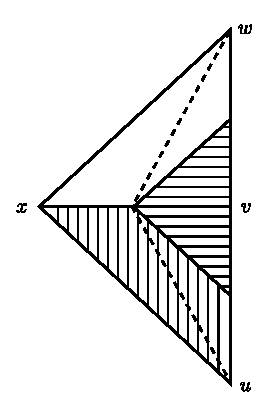
\includegraphics{figure/fig17.eps}
\end{figure}\pageoriginale

[The picture is actually the union of the two triangles $[x,v,w]$ and $[x,v,u]$ in $C(P)$, which we have flattened out to put in a planar picture. The vertically shaded part is the porition of $L\times[\frac{1}{2},1]$ in the cross section and the horizontally shaded part is the part of $C_{\frac{1}{2}}(P)$ in the cross section. We have to push the union of these two into the vertically shaded portion, and this uniformly over all cross sections].

From this picture we may see the following: $C(P)$ is the union of 
\begin{align*}
A &= \left\{X\times\left[\frac{1}{2},1\right]\right\}\ast\{u,w\},\quad\text{and}\\
B &= \left\{X\times\frac{1}{2}\right\}\ast J\quad\text{where}\quad J=v\ast\{u,w\}.\\
\text{And}\quad A\cap B &= \left\{X\times\frac{1}{2}\right\}\ast \{u,w\}.
\end{align*}

Now $J$ is just, polyhedrally, an interval, and so there is obviously a polyhedral equivalence $f:J\to J$ such that 
\begin{align*}
& f(u)=u,f(w)=w\\
& f(\frac{1}{2}v+\frac{1}{2}w)=\frac{1}{2}v+\frac{1}{2}u.
\end{align*}

Such an $f$ will take the part $[u,v]\cup [v,\frac{1}{2}v+\frac{1}{2}w]$ onto $[u,\frac{1}{2}u+\frac{1}{2}v]$.

Let $g:B\to B$ be the join of $f$ on $J$ and identity on $X\times \frac{1}{2}$. It is clear that $g|A\cap B$ is the identity map, and so by extending by identity on $A$, we get a polyhedral equivalence say\pageoriginale $h:C(P)\to C(P)$.

It should be pictorially evident that $h$ has the desired properties.
\end{proof}

Putting all these together we get the proposition which we need:

\begin{proposition}\label{chap6-prop6.8.5}
{\em Hypotheses:}
\begin{enumerate}
\renewcommand{\labelenumi}{\rm(\theenumi)}
\item $\mathscr{P}$ is a simplicial presentation of $P$, $C(P)$ the cone over $P$ with vertex $v$, $C(\mathscr{P})=\mathscr{P}\ast\{\{v\}\}$, and $\sum$ a set of vertices of $\mathscr{P}$.

\item There is a polyhedron $X$ and a polyhedral equivalence $h:P\to X\ast \{u,w\}$ such that $h(|\mathscr{P}_{\sum}|)=Y\ast u$, for some $Y\subset X$.

\item $|\delta_{\mathscr{C}(\mathscr{P})}v|$ and $\delta_{C(\mathscr{P})}(\sum)$ are constructed with reference to some centering $\mathscr{V}$ of $C(\mathscr{P})$.
\end{enumerate}
\end{proposition}

\noindent
{\bf Conclusion:}~ There is a polyhedral equivalence $\alpha:C(P)\to C(P)$ such that $\alpha|P=\text{id}_{P}$ and $\alpha$ maps $(\delta_{C(\mathscr{P})}(\sum))\cup (\delta_{\mathscr{C}(\mathscr{P})}v|$ onto $(\delta_{C(\mathscr{P})}(\sum))$.

\begin{proof}
Let $\eta$ be the centering of $C(\mathscr{P})$ described in
proposition \ref{chap6-prop6.8.3}. Let $f=f_{\eta,\mathscr{V}}$ be the
simplicial isomorphism of $d(C(\mathscr{P}),\mathscr{V})$ onto\break
$d(C(\mathscr{P}),\eta)$. 

Let $h_{1}:C(P)\to C(X\ast\{u,w\})$ be the join of $h:P\to X\ast \{u,w\}$ and the map vertex to vertex.

Now $\delta_{\mathscr{P}}(\sum)$ is a regular neighbourhood of $|\mathscr{P}_{\sum}|$ in $P$, and therefore $hf(\delta_{\mathscr{P}}(\sum))$ is a regular neighbourhood $hf(|\mathscr{P}_{\sum}|)$ in $X\ast \{u,w\}$. But $f(|\mathscr{P}_{\sum}|)=|\mathscr{P}_{\sum}|$ - infact $f$ maps every $\mathscr{P}$-simplex onto itself - and $h(|\mathscr{P}_{\sum}|)= \gamma \ast u$. Thus\pageoriginale $hf(\delta_{\mathscr{P}}(\sum))$ is a regular neighbourhood of $Y\ast u$ in $X\ast \{u,w\}$. Therefore by \ref{chap6-prop6.8.2}, $hf(\delta_{\mathscr{P}}(\sum))$ is a regular neighbourhood of $u$ in $X\ast\{u,w\}$. But so is $X\ast u$. Hence there is a polyhedral equivalence $\beta:X\ast \{u,w\}\to X\ast \{u,w\}$ such that
$$
\beta(hf(\delta_{\mathscr{P}}(\sum)))=X\ast u.
$$

Let $\beta_{1}:C(X\ast \{u,w\})\to C(X\ast \{u,w\})$ be the join of and identity map of the vertex of the cone.

Now $f$ is such that
$f(\delta_{C(\mathscr{P})}(\sum))=f(\delta_{\mathscr{P}}(\sum))\times[\frac{1}{2},1]$
and $f(|\delta_{C(\mathscr{P})}\break v|)=C_{\frac{1}{2}}(P)$. 

Since $\beta_{1}$ and $h_{1}$ are radial extensions the same thing holds, i.e.
\begin{align*}
\beta_{1}h_{1}f(\delta_{(C|\mathscr{P})}(\sum)) &= \beta_{1}h_{1}(f(\delta_{\mathscr{P}}(\sum))\times [\frac{1}{2},1]\\
&= \beta hf(\delta_{\mathscr{P}}(\sum))\times[\frac{1}{2},1]
\end{align*}
which is $\{X\ast u\}\times [\frac{1}{2},1]$, and
\begin{align*}
\beta_{1}h_{1}f(|\delta_{C(\mathscr{P})}v|) &= \beta_{1}h_{1}(C_{\frac{1}{2}}(P))\\
&= C_{\frac{1}{2}}(X\ast \{u,w\}).
\end{align*}

Applying \ref{chap6-prop6.8.4}, we get a polyhedral equivalence
$$
\gamma:C(X\ast\{u,w\})\to C(X\ast \{u,w\})\quad\text{with}\quad \gamma|X\ast\{u,w\}=
$$
identity and
\begin{gather*}
\gamma \left((X\ast u)\times[\frac{1}{2},1]\cup C_{\frac{1}{2}}(X\ast\{u,w\})\right)\\
=(X\ast u)\times[\frac{1}{2},1].
\end{gather*}

The desired map $\alpha$ is now,
$$
\alpha=f^{-1} \circ h^{-1}_{1} \circ \beta_{1}^{-1} \circ \gamma \circ \beta_{1} \circ h_{1} \circ f.
$$
\end{proof}

We\pageoriginale will now write down two specific corollaries of proposition 
\ref{chap6-prop6.8.5}, which will immediately give the regular neighbourhood theorem. First we recall the notation at the end of section 3 
(\ref{chap6-sec6.3.10}).

If $\mathscr{P}$ is regular presentation, given a centering $\eta$ of $\mathscr{P}$ and a centering of $d(\mathscr{P},\eta)$, we defined 
$$
C^{*}=|\delta_{d\mathscr{P}}(\eta C)|,\quad\text{for any}\quad C
$$
and $\mathscr{N}^{*}=\cup\{C^{*}|C\in\mathscr{N}\}$, for any subset $\mathscr{N}$ of $\mathscr{P}$. If $\mathscr{N}$ is a subpresentation of $\mathscr{P}$, then $d(\mathscr{N},\eta)$ (where $\eta|\mathscr{N}$ is again denoted by $\eta$) is full in $d(\mathscr{P},\eta)$. Writing $\mathscr{N}'=d(\mathscr{N},\eta)\mathscr{P}'=d(\mathscr{P},\eta)$, and $\sum$ as the set of vertices of $\mathscr{P}'$ of the form $\eta C$, for $C\in \mathscr{N}$, we see that $\mathscr{P}'_{\sum}=\mathscr{N}'$ and $\delta_{\mathscr{P}'}(\sum)=\mathscr{N}^{\ast}$, which is a regular neighbourhood of $|\mathscr{N}|$ in $|\mathscr{P}|$.

\begin{corollary}\label{chap6-coro6.8.6}
Let $\mathscr{P}$ be a regular presentation with a subpresentation $\mathscr{N}$, $E$ a free edge of $\mathscr{N}$ with attaching membrane $A$ such that $(E,A)$ is homogeneous in $\mathscr{P}$. Then there is a polyhedral equivalence $h=|\mathscr{P}|\to |\mathscr{P}|$ which is identity outside of $\overline{E}\ast |\lambda_{\mathscr{P}}E|$ and which takes $\mathscr{N}^{*}$ onto $(\mathscr{N}-\{E\})^{\ast}$. 

\medskip
\noindent
[Note: It is understood that there is a centering $\eta$ of $\mathscr{P}$, and a centering of $d(\mathscr{P},\eta)$].
\end{corollary}

\begin{proof}
Look at $St(\eta E, d\mathscr{P})$; this is a presentation say $\mathscr{P}'$ of $\overline{E}\ast |\lambda_{\mathscr{P}}E|$. Let $\sum$ denote the set of vertices of $d\mathscr{P}$ of the form $\eta F$ for $F<E$ and $\eta A$. Then $|\mathscr{P}'_{\sum}|$ is the join of $\p E$ to $\eta A$. Since $|\lambda_{\mathscr{P}}E|$ is equivalent to a suspension (homogenity\pageoriginale of $(E,A)$) with $\eta A$ going to a pole, we see that $\p E\ast |\lambda_{\mathscr{P}}E|$ is equivalent to a suspension with $|\mathscr{P}'_{\sum}|$ going to a subcone. And $\overline{E}\ast|\lambda_{\mathscr{P}}E|$ is a cone over $\p E\ast |\lambda_{\mathscr{P}}E|$. And consider the centering of $\mathscr{P}'$ coming from that of $d(\mathscr{P},\eta)$. 


Thus we have the situation of \ref{chap6-prop6.8.5}, and making the necessary substitutions in \ref{chap6-prop6.8.5}, we get a polyhedral equivalence 
$\alpha$ of $|\mathscr{P}'|=\overline{E}\ast |\lambda_{\mathscr{P}}E|$ taking $|\delta'_{\mathscr{P}}(\eta E)|\cup \delta_{\mathscr{P}'}(\sum)$ onto $\delta_{\mathscr{P}'}(\sum)$. $|\delta_{\mathscr{P}'}(\eta E)|$ is just $E^{\ast}$. Now observe that the set of centres of elements of $\mathscr{N}$ in $\mathscr{P}'$ is $\sum\cup\{\eta E\}$. (This is where we use the fact that $E$ is a free edge). Therefore $\mathscr{N}^{\ast}\cap |\mathscr{P}'|=E^{\ast}\cup \delta_{\mathscr{P}'}(\sum)$ and $(\mathscr{N}-\{E\})^{\ast}\cap |\mathscr{P}'|=\delta_{\mathscr{P}'}(\sum)$. So $\alpha$ takes the part of $(\mathscr{N}^{\ast})$ in $|\mathscr{P}'|$ onto the part of $(\mathscr{N}-\{E\})^{\ast}$ in $|\mathscr{P}'|$. $\alpha$ is identity on the base of the cone, and $E^{\ast}\subset |\mathscr{P}'|$. Therefore extending $\alpha$ to an equivalence $h$ of $|\mathscr{P}|$ by patching up with identity outside 
$|\mathscr{P}'|$, we see that $h$ takes $\mathscr{N}^{\ast}$ onto $(\mathscr{N}-\{E\})^{\ast}$ and is identity outside $|\mathscr{P}'|=\overline{E}\ast|\lambda_{\mathscr{P}}E|$. 
\end{proof}

\begin{corollary}\label{chap6-coro6.8.7}
In the same situation, there is a polyhedral equivalence $h':|\mathscr{P}|\to |\mathscr{P}|$ which is identity outside $\overline{A}\ast |\lambda_{\mathscr{P}}A|$, which takes $(\mathscr{N}-\{E\})^{\ast}$ onto $(\mathscr{N}-\{E,A\})^{\ast}$.

[for this corollary we need only that $E$ is a free edge of $A$, and $A$ is the attaching membrane. Homogenity of $(E,A)$ is not necessary].
\end{corollary}

\begin{proof}
This time we call $\mathscr{P}'=St(\eta A,d\mathscr{P})$, and $\sum$ the set of vertices $\eta F$, $F<A$ and $F\neq E$. Then $|\mathscr{P}'_{\sum}|=\p A-E$. $\p A$ is equivalent to a suspension with $\p A-E$ as the lower hemisphere. Hence\pageoriginale 
$\p A\ast |\lambda_{\mathscr{P}}A|$ is equivalent to a suspension with $|\mathscr{P}'_{\sum}|$ mapping onto a subcone. Applying \ref{chap6-prop6.8.5}, we get a polyhedral equivalence $\alpha'$ of $\overline{A}\ast |\lambda_{\mathscr{P}}A|$ on itself, which is identity on $\p A\ast |\lambda_{\mathscr{P}}A|$ and takes $\delta_{\mathscr{P}'}(\sum)\cup A^{\ast}$ onto $\delta_{\mathscr{P}'}(\sum)$. Since $E$ is a free edge and $A$ is principal in $\mathscr{N}$, $\delta_{\mathscr{P}'}(\sum)$ is just the part of $(\mathscr{N}-\{E,A\})^{\ast}$ in $\overline{A}\ast |\lambda_{\mathscr{P}}A|$, and $\delta_{\mathscr{P}'}(\sum)\cup A^{\ast}$ is the part of $(\mathscr{N}-\{E\})^{\ast}$ in $\overline{A}\ast |\lambda_{\mathscr{P}}A|$. Extending $\alpha'$ to an equivalence $h'$ of $|\mathscr{P}|$ by patching up with identity outside $\overline{A}\ast |\lambda_{\mathscr{P}}A|$, since $A^{\ast}$ is contained in $\overline{A}\ast|\lambda_{\mathscr{P}}A|$ we see that $h'$ takes $(\mathscr{N}-\{E\})^{\ast}$ onto $(\mathscr{N}-\{E,A\})^{\ast}$ and is identity outside $\overline{A}\ast|\lambda_{\mathscr{P}}A|$.
\end{proof}

Thus in the situation of \ref{chap6-coro6.8.6}, if we take the composition $h'h$ of the equivalences given by \ref{chap6-coro6.8.6} and \ref{chap6-coro6.8.7}, $h'\circ h$ takes $\mathscr{N}^{\ast}$ onto $(\mathscr{N}-\{E,A\})^{\ast}$. Support of $h'\subset \overline{A}\ast |\lambda_{\mathscr{P}}A|$, support of $h\subset\overline{E}\ast|\lambda_{\mathscr{P}}E|$, hence $h'\circ h$ fixes, the polyhedron $|(\mathscr{N}-\{E,A\})|$. This at once gives,

\begin{proposition}\label{chap6-prop6.8.8}
If $\mathscr{N}\searrow \mathscr{X}$ homogeneously in $\mathscr{P}$, then there is a polyhedral equivalence of $|\mathscr{P}|$, which is identity on $|\mathscr{X}|$ and takes $\mathscr{N}^{\ast}$ onto $\mathscr{X}^{\ast}$.
\end{proposition}

\begin{corollary}\label{chap6-coro6.8.9}
If $N\searrow X$ homogeneously in $P$, then any regular neighbourhood of $N$ in $P$ is a regular neighbourhood of $X$ in $P$.
\end{corollary}


\noindent
{\bf Proof of the regular neighbourhood theorem \ref{chap6-sec6.8.1}.}

By \ref{chap6-coro6.8.9} any regular neighbourhood say $N'$ of $N$ is a regular neighbourhood of $X$. Since $N$ is bicollared in $P$, there is a polyhedral equivalence $h$ of $P$ taking $N$ onto $N'$. Since $X\subset \Int_{P}N$, $h$ can be chosen to be fixed on $X$ (see \ref{chap6-ex6.4.8}). Therefore $N$ is a regular neighbourhood of $X$.

\section{Some applications and remarks}\pageoriginale\label{chap6-sec6.9}

In this section we make a few observations about the previous concepts in the context of $PL$-manifolds

\subsection{}\label{chap6-sec6.9.1}
Let $M$ be a $PL$-manifold, $\p M$ its boundary, $\mathscr{P}$ a regular presentation of $M$. Let $E$, $A\in \mathscr{P}$, $E<A$ and $\dim A=\dim E+1$. $(E,A)$ is homogeneous in $\mathscr{P}$ if and only if either both $E$ and $A$ are in $\p M$ or both $E$ and $A$ are in $M-\p M$.

\begin{proof}
Let $\eta$ be a centering of $\mathscr{P}$. Let $E'\subset E$ a simplex of $d(\mathscr{P},\eta)$ of dimension $=\dim E$, and $A'=\{\eta A\}E'$. Now the problem is equivalent to: When is $|LK(E',d\mathscr{P})|$ equivalent to a suspension with $\eta A$ going to a vertex? If $E$ and $A$ are in $M-\p M$, so are $E'$ and $A'$ and $|LK(E',d\mathscr{P})|$ is a sphere, hence it is possible. If $E$ and $A$ are both in $\p M$, so are $E'$ and $A'$ and $|Lk(E',d\mathscr{P})|$ is a cell, with $\eta A$ contained in the boundary. So again it is possible. If $E$ is in $\p M$ and $A$ is in $M-\p M$ so are $E'$ and $A'$ and $|Lk(E',d\mathscr{P})|$ is a cell with $\eta A$ in the interior. Hence in this case it is impossible.
\end{proof}

Suppose now that $\mathscr{N}$ and $\mathscr{X}$ are subpresentation of $\mathscr{P}$ and $\mathscr{N}\searrow \mathscr{X}$ homogeneously in $\mathscr{P}$. In the sequence of (elementary) homogeneous of collapses from $\mathscr{N}$ to $\mathscr{X}$, if a collapse $C_{1}$ in the boundary comes before a collapse $C_{2}$ in the interior we can interchange them i.e.\@ if $\mathscr{N}_{i-1}\searrow^{C_{1}}\mathscr{N}_{i}\searrow^{C_{2}}\mathscr{N}_{i+1}$, then we can find $\mathscr{N}'_{i}$ such that $\mathscr{N}_{i-1}\searrow^{C'_{2}}\mathscr{N}'_{i}\searrow^{C'_{1}}\mathscr{N}_{i+1}$ and the free edge and attaching membrane of $C_{i}$ and $C'_{i}$, $j=1,2$ are the same. Doing this a finite number of times we have

\subsection{}\label{chap6-sec6.9.2}
If\pageoriginale $N\searrow X$ homogeneously in $M$, then $N\searrow X\cup (N\cap \p M)\searrow X$. In particular, this is true for regular neighbourhoods. Some rearrangement is possible for the usual elementary collapses also:

\setcounter{proposition}{2}
\begin{ex}\label{chap6-ex6.9.3}
Suppose $\mathscr{P}\searrow \mathcal{Q}$, combinatorially, and $\mathscr{P}_{1},\ldots,\mathscr{P}_{k}$, $1\leq i\leq k$ are subpresentations such that $\mathscr{P}_{i}$ is obtained from $\mathscr{P}_{i-1}$ by an elementary collapse at the free edge $E_{i-1}$ with attaching membrane $A_{i-1}$ and $\mathscr{P}=\mathscr{P}_{1}$, $\mathcal{Q}=\mathscr{P}_{k}$. Then we can find subpresentations $\mathscr{P}'_{1}$, $\mathscr{P}'_{2},\ldots,\mathscr{P}'_{k}$, $\mathscr{P}'_{1}=\mathscr{P}$, $\mathscr{P}'_{k}=\mathcal{Q}$, such that $\mathscr{P}'_{i}$ is obtained from $\mathscr{P}'_{i-1}$ by an elementary collapse at the free edge $E'_{i-1}$ with attaching membrane $A'_{i-1}$ and $\dim A'_{i}\geq \dim A'_{i-1}$. Moreover, except for order, the pairs $(E'_{i},A'_{i})$ are the same as the pairs $(E_{j},A_{j})$.

More briefly, we can rearrange the collapses in the order of non-increasing dimension.
\end{ex}

\begin{ex}\label{chap6-ex6.9.4}
An $n$-cell collapses to any $(n-1)$-cell in its boundary. This follows from \ref{chap6-ex6.5.10}.
\end{ex}

\begin{ex}\label{chap6-ex6.9.5}
An $n$-cell is collapsible to any point in it.
\end{ex}

We call polyhedron {\em collapsible} if it collapses to a point.

\setcounter{proposition}{4}
\begin{dashex}\label{chap6-dashex6.9.5}
A collapsible polyhedron collapses to any point in it. 

[Hint: By virtue of \ref{chap6-ex6.9.3}, it is enough to consider one dimensional collapsible presentations with the given point as a vertex].
\end{dashex}

\setcounter{subsection}{5}
\subsection{}\label{chap6-sec6.9.6}
If $M$ is a collapsible $PL$ $n$-manifold, then $M$ is a $n$-cell.

\medskip
\noindent
{\bf Sketch of the proof:}~ $\p M\neq \emptyset$, for if $\p M=\emptyset$, there is no free edge to start the collapsing. Next we can assume that $M$ collapses to a point in $M-\p M$, either by \ref{chap6-dashex6.9.5}$'$ or by \ref{chap6-ex6.9.4} and \ref{chap6-ex6.5.11}. Now attach\pageoriginale a collar of $\p M$ to $M$ (to get $PL$-manifold $M'$) so that all the collapsing is in the interior of $M'$, hence homogeneous. Now all the conditions of the regular neighbourhood theorem are satisfied. Hence $M$ is the regular neighbourhood of a print in $M'$, hence an $n$-cell.

The following two remarks will be useful in the next chapter.

\subsection{}\label{chap-sec6.9.7}
Let $f:K\times D^{n-k}\to M^{n}$ be an imbedding into int $M$, where $K$ is a $K$-manifold and $D^{n-k}$ an $(n-k)$-cell. Then $f(K\times D^{n-k})$ can be shrunk into any given neighbourhood of $f(K\times e)$ in $M$, for a fixed $e\in \text{int\,}D^{n-k}$ by an isotopy which can be assumed to be fixed on $f(K\times e)$.

$K\times D^{n-k}\searrow K\times e$ (this follows, for example, from \ref{chap6-ex6.5.14} by induction). It is easily seen that $f(K\times D^{n-k})$ is a neighbourhood of $f(k\times e)$ in $M$ and is bicollared.

\setcounter{proposition}{7}
\begin{proposition}\label{chap6-prop6.9.8}
Let $M$ be a $PL$ $n$-manifold, and $N$ a $PL$ $(n-1)$-manifold in $\p M$, and $M\searrow N$. Then $M$ is polyhedrally equivalent to $N\times I$. Moreover the polyhedral equivalence $h:M\approx N\times I$, can be so chosen that $h(n)=(n=0)$ for $n\in N$. 
\end{proposition}

\begin{proof}
Such an $N$ cannot be the whole of $\p M$. Either $\p N\neq \emptyset$, or $N$ is a finite union of components of $\p M$ (see \ref{chap4-ex4.4.16}). In any case $N$ is bicollared in $\p M$. If $N'$ is regular neighbourhood of $N$ in $\p M$, since $N$ is bicollared in $\p M$, $N'$ is polyhedrally equivalent to $N$ (\ref{chap6-ex6.4.8}).

Since $M\searrow N$, there is a regular neighbourhood say $A$ of $N$ in $M$ such that $M\searrow A$ (see \ref{chap6-ex6.6.9}). Let $A\cap \p M=N'$. Then $N'$ is a regular neighbourhood of $N$ in $\p M$. It is clear that\pageoriginale $A$ is polyhedrally equivalent to $N\times I$. Now attach $B$ and $C$, $B$ a collar over $\overline{\p M-N'}$ and $C$ a collar over $N$ to $M$ such that $B\cap C=\emptyset$. Let the resulting manifold be $M'$.
\begin{figure}[H]
\centering
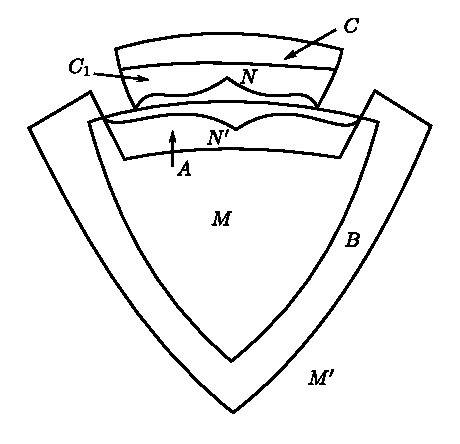
\includegraphics{figure/fig18.eps}
\end{figure}

Consider another collar $C_{1}\subset C$, and the manifolds $A\cup C_{1}$ and $M\cup C_{1}$. In $M'$, all the collapses from $M$ to $A$ are in the interior and hence $M\searrow A$ homogeneously in $M'$, and the collapsing from $A\searrow N$ continues to be homogeneous in $M$. Clearly $C_{1}\searrow N$ homogeneously in $M'$. Thus both $A\cup C_{1}$ and $M\cup C_{1}$ collapse homogeneously in $M'$ to $N$, both are neighbourhoods of $N$ in $M'$ and both are bicollared. Hence there is an equivalence $A\cup C_{1}\approx M\cup C_{1}$. Clearly $A\cup C_{1}\approx N\times I$. Hence $M\cup C_{1}\approx N\times I$, hence $M\approx N\times I$.

To prove the last remark observe that if $\mathscr{L}:N\times I\approx C_{1}$ is an equivalence such that $\mathscr{L}(n,1)=n$, for $n\in N$, the equivalence $M\approx M\cup C_{1}$ can be chosen such that it carries $n\in N$ to $\mathscr{L}(n,0)\in C_{1}$. Finally the equivalence $A\cup C_{1}\approx M\cup C_{1}$ can be assumed to be identity on $C_{1}$.
\end{proof}

\section{Conclusion}\pageoriginale\label{chap6-sec6.10}

Now let us, recaptitulate briefly the programme for proving the regular neighbourhood theorem:
\begin{itemize}
\item[(A)] We have a notion of equivalence of pairs
$$
(P,X)\approx (P',X')
$$

\item[(B)] We define a regular neighbourhood of $X$ in $P$ to be any thing equivalent by an auto-equivalence of $(P,X)$ to $|N_{\mathscr{P}}(\mathscr{X})|$, where $\mathscr{P}$ is a simplicial presentation of $P$ with a full subpresentation $\mathscr{X}$ covering $X$.

\item[(C)] We have the notions of the cone on $P$, suspension on $P$, and $P\times I$; and hence the idea of local collaring, collaring and bicollaring.

\item[(D)] We can prove: We can prove: $P\times[0,\frac{1}{2}]$ is a regular neighbourhood of $P\times 0$ in $P\times [0,1]$. The lower half of the suspension of $P$ is a regular neighbourhood of a pole. A locally collared subpolyhedron is collared. Regular neighbourhood of a pole. A locally collared subpolyhedron is collared. Regular neighbourhoods are bicollared. 

\item[(E)] We have for regular presentations, the notion of collapsing, and of homogeneous; and we prove that $N\searrow X$ homogeneously in $P$ if $N$ is a regular neighbourhood of $X$ in $P$.

\item[(F)] Finally, we prove the converse, that if $N\searrow X$ homogeneously in $P$, then a regular neighbourhood of $N$ is a regular neighbourhood of $X$. We pick up a particular regular neighbourhood of $N$ and strink it down a bit at a time to a particular regular neighbourhood of $X$. In doing this, we need to have proved the theorem for a particular case: $X'$ is a pole of a suspension $P'$ and\pageoriginale $N'$ is a subcone of $P'$. An analysis of the proof shows that we need the result for various $P'$ of dimension less than that of $P$. Hence we could have proved this by induction on dimension, although it is simple enough to prove in the special case by construction.
\end{itemize}

Now it should be remarked that precisely the same programme can be carried out in other contexts. In particular for pairs:

A pair $(P,Q)$ is a polyhedron $P$ with a subpolyhedron $Q$; we say $(P_{1},Q_{1})\subset (P_{2},Q_{2})$ if $P_{1}\subset P_{2}$, and $Q_{1}=Q_{2}\cap P_{1}$. If $(P_{1},Q_{1})\subset (P_{2},Q_{2})$ we define the boundary of the former in the latter to be $(bd_{P_{2}}P_{1},Q_{1}\cap bd_{P_{2}}P_{1})$.

Define an equivalence $h:(P_{1},Q_{1})\to (P_{2},Q_{2})$ to be a polyhedral equivalence $\alpha:P_{1}\approx P_{2}$ mapping $Q_{1}$ onto $Q_{2}$.

An admissible presentation of $(P,Q)$ is a pair of regular presentations $\mathcal{Q}\subset\mathscr{P}$ with $|\mathscr{P}|=P$, $|\mathcal{Q}|=Q$. A free edge of an admissible presentation $(\mathscr{P},\mathcal{Q})$ is an $E\in \mathscr{P}$, which is a free edge of $\mathscr{P}$ with attaching membrane $A$, such that if $E\in \mathcal{Q}$, then $A\in \mathcal{Q}$.

The programme can be carried out mechanically with the obvious definition of homogeneous collapsing.

Finally, we draw some consequences, by applying to $PL$-manifolds.

Let $A\subset B$, where $A$ is a $PL$ $a$-manifold and $B$ is a $PL$ $b$-manifold. We say $(B,A)$ is locally {\em un-knotted} if, for every $x\in A$, if $(L_{B},L_{A})$ is polyhedrally equivalent to $(L_{A}\ast X,L_{A})$ for\pageoriginale some $X$. It is possible to show that $X$ must be either a cell or a sphere of dimension $b-a-1$; and that if $A$ is connected, then either all the $X$'s are cells, in which case $A$ is locally un-knotted in $\p B$ or all $X$'s are spheres, in which case $\p A=A\cap \p B$.

It then occurs as in the case of a single manifold, that all the collapsing (in the pair sense) which is in the interior of $(B,A)$ is homogeneous, and hence we can prove the following result:

Let $D^{a}\subset \Delta^{b}$, with $(\Delta,D)$ a locally un-knotted pair of the sort where $\p D=D\cap \p \Delta$. Then if $\Delta\searrow D\searrow$ point, the pair $(\Delta,D)$ is an absolute regular neighbourhood of a point (relative to $(\p \Delta,\p D)$ and so $(\Delta,D)$ is polyhedrally equivalent to $(S\ast D,D)$ where $S$ is a $(b-a-1)$-sphere, i.e.\@ $(\Delta,D)$ is un-knotted.

[This is a key lemma for Zeeman's theorem, that $(b-a)\geq 3\Rightarrow (\Delta,D)$ is un-knotted. See Zemman ``Seminar on combinatorial Topology'', Chapter IV, pp.\@ 4-5]. 






